% Options for packages loaded elsewhere
\PassOptionsToPackage{unicode}{hyperref}
\PassOptionsToPackage{hyphens}{url}
%
\documentclass[
  10pt,
  onecolumn]{article}
\usepackage{amsmath,amssymb}
\usepackage{lmodern}
\usepackage{setspace}
\usepackage{iftex}
\ifPDFTeX
  \usepackage[T1]{fontenc}
  \usepackage[utf8]{inputenc}
  \usepackage{textcomp} % provide euro and other symbols
\else % if luatex or xetex
  \usepackage{unicode-math}
  \defaultfontfeatures{Scale=MatchLowercase}
  \defaultfontfeatures[\rmfamily]{Ligatures=TeX,Scale=1}
  \setmainfont[]{Arial}
  \setmonofont[]{Times New Roman}
\fi
% Use upquote if available, for straight quotes in verbatim environments
\IfFileExists{upquote.sty}{\usepackage{upquote}}{}
\IfFileExists{microtype.sty}{% use microtype if available
  \usepackage[]{microtype}
  \UseMicrotypeSet[protrusion]{basicmath} % disable protrusion for tt fonts
}{}
\makeatletter
\@ifundefined{KOMAClassName}{% if non-KOMA class
  \IfFileExists{parskip.sty}{%
    \usepackage{parskip}
  }{% else
    \setlength{\parindent}{0pt}
    \setlength{\parskip}{6pt plus 2pt minus 1pt}}
}{% if KOMA class
  \KOMAoptions{parskip=half}}
\makeatother
\usepackage{xcolor}
\usepackage[left=0.8in,right=0.8in,top=0.8in,bottom=0.5in]{geometry}
\usepackage{graphicx}
\makeatletter
\def\maxwidth{\ifdim\Gin@nat@width>\linewidth\linewidth\else\Gin@nat@width\fi}
\def\maxheight{\ifdim\Gin@nat@height>\textheight\textheight\else\Gin@nat@height\fi}
\makeatother
% Scale images if necessary, so that they will not overflow the page
% margins by default, and it is still possible to overwrite the defaults
% using explicit options in \includegraphics[width, height, ...]{}
\setkeys{Gin}{width=\maxwidth,height=\maxheight,keepaspectratio}
% Set default figure placement to htbp
\makeatletter
\def\fps@figure{htbp}
\makeatother
\setlength{\emergencystretch}{3em} % prevent overfull lines
\providecommand{\tightlist}{%
  \setlength{\itemsep}{0pt}\setlength{\parskip}{0pt}}
\setcounter{secnumdepth}{-\maxdimen} % remove section numbering
\newlength{\cslhangindent}
\setlength{\cslhangindent}{1.5em}
\newlength{\csllabelwidth}
\setlength{\csllabelwidth}{3em}
\newlength{\cslentryspacingunit} % times entry-spacing
\setlength{\cslentryspacingunit}{\parskip}
\newenvironment{CSLReferences}[2] % #1 hanging-ident, #2 entry spacing
 {% don't indent paragraphs
  \setlength{\parindent}{0pt}
  % turn on hanging indent if param 1 is 1
  \ifodd #1
  \let\oldpar\par
  \def\par{\hangindent=\cslhangindent\oldpar}
  \fi
  % set entry spacing
  \setlength{\parskip}{#2\cslentryspacingunit}
 }%
 {}
\usepackage{calc}
\newcommand{\CSLBlock}[1]{#1\hfill\break}
\newcommand{\CSLLeftMargin}[1]{\parbox[t]{\csllabelwidth}{#1}}
\newcommand{\CSLRightInline}[1]{\parbox[t]{\linewidth - \csllabelwidth}{#1}\break}
\newcommand{\CSLIndent}[1]{\hspace{\cslhangindent}#1}
\ifLuaTeX
  \usepackage{selnolig}  % disable illegal ligatures
\fi
\IfFileExists{bookmark.sty}{\usepackage{bookmark}}{\usepackage{hyperref}}
\IfFileExists{xurl.sty}{\usepackage{xurl}}{} % add URL line breaks if available
\urlstyle{same} % disable monospaced font for URLs
\hypersetup{
  pdftitle={Nitric-oxide-feedback to ciliary photoreceptor cells orchestrates UV avoidance in zooplankton},
  hidelinks,
  pdfcreator={LaTeX via pandoc}}

\title{Nitric-oxide-feedback to ciliary photoreceptor cells orchestrates
UV avoidance in zooplankton}
\author{true}
\date{}

\begin{document}
\maketitle

\setstretch{1.2}
\hypertarget{abstract}{%
\subsection{Abstract}\label{abstract}}

Nitric oxide (NO) generated by nitric-oxide synthase (NOS) is a key
regulator of animal physiology. Here we uncover a role for NO in shaping
circuit dynamics to orchestrate light-avoidance behaviour. We studied
UV-avoidance mediated by brain ciliary photoreceptors (cPRCs) in larval
\emph{Platynereis dumerilii}, a marine annelid. We found NOS
specifically expressed in interneurons (INNOS) postsynaptic to cPRCs.
Stimulation of cPRCs by violet light leads to cPRC inhibition but
concomitant INNOS activation and NO production. NO feeds back to cPRCs
and triggers their delayed activation through an unconventional guanylyl
cyclase. This results in the activation of projection interneurons and
the inhibition of serotonergic ciliomotor neurons. In \emph{NOS}
mutants, NO feedback and projection-neuron activation do not occur and
avoidance behaviour is defective. By mathematical modelling, we could
capture the circuit dynamics in both wild-type and mutant larvae. Our
results reveal how NO-mediated neuroendocrine signalling gates a
synaptic circuit to initiate light-avoidance behaviour.

\hypertarget{introduction}{%
\subsection{Introduction}\label{introduction}}

Neuronally produced nitric oxide (NO) can act as a diffusible
neuromodulator. This small free-radical molecule is synthesized by
nitric oxide synthase (NOS)\ldots{}

In the mammalian retina, NO is produced by amacrine cells and activates
a \emph{soluble guanylate cyclase (sGC)} in cone bipolar cells. The
NO-dependent increased in cGMP tunes bipolar cell activity \ldots.
{[}refs{]} {[}other examples{]}

To investigate NO signalling in the modulation of neural circuit
dynamics, we studied the larval stages of the marine annelid model
\emph{Platynereis dumerilii} (Ozpolat et al., 2021). We uncovered an
essential function for NO in these larvae in UV/violet-light avoidance.
In \emph{Platynereis} larvae, UV/violet avoidance is characterised by
downward swimming and is mediated by the UV/violet-responding brain
ciliary photoreceptor cells (cPRCs).

The cPRCs express a vertebrate-type ciliary opsin, c-opsin1 (Arendt et
al., 2004). This opsin forms a UV-absorbing bistable photopigment with
an absorption maximum around 384 nm Verasztó et al. (2018).
\emph{c-opsin1} knockout larvae show defective UV/violet avoidance
(Verasztó et al., 2018). Here we show that \emph{Platynereis} \emph{NOS}
is expressed in interneurons of the cPRC circuitry and is required for
UV/violet-avoidance behaviour. By combining calcium imaging across the
fully-mapped cPRC circuit, genetic perturbations and mathematical
modelling, we describe how NO tunes circuit dynamics through
non-synaptic reverse signalling to cPRCs. This delayed neuroendocrine
feedback is essential for circuit output, and integrates UV/violet input
and also induces a short-term memory manifest in altered circuit
activity.

\#In adult worms, UV light and c-opsin1 modulate locomotion and
maturation (Veedin Rajan et al., 2021).

\hypertarget{results}{%
\subsection{Results}\label{results}}

\textbf{Nitric oxide synthase is expressed in interneurons of the
UV-avoidance circuit}

We identified a single \emph{nitric oxide synthase} (\emph{NOS}) gene in
the \emph{Platynereis dumerilii} genome and transcriptome data.
Phylogenetic analysis of NOS proteins indicate that \emph{Platynereis}
NOS belongs to an orthology group of metazoan NOS sequences
\textbf{(Figure 1---figure supplement 1)}. To characterise the
expression pattern of \emph{NOS} we used in situ hybridization chain
reaction (HCR) and transient transgenesis. In two- and three-day-old
larvae, we detected \emph{NOS} expression in four cells (two of them
weakly expressing) in the apical organ region \textbf{(Figure 1D and
Figure 1---figure supplement 2)}. \emph{NOS} was also expressed in the
region of the visual eyes (adult eyes) and the pigmented eyespots
\textbf{(Figure 1---figure supplement 1)}. The four apical organ cells,
but not the eyes, were also labelled with a \emph{NOS} reporter
construct driving palmitoylated-tdTomato \textbf{(Figure 1E)}. This
reporter also revealed the axonal projections of these central
NOS-expressing neurons. The position and morphology of the four
\emph{NOS+} cells allowed us to identify the same four cells as four
interneurons (INNOS) in our three-day-old whole-body \emph{Platynereis}
volume EM data (Verasztó et al., 2020; Williams et al., 2017)
\textbf{(Figure 1B,C)}. In the synaptic connectome, the INNOS cells are
postsynaptic to the UV-sensory cPRCs and presynaptic to the INRGW
interneurons, which are also cPRC targets \textbf{(Figure 1C,F)}. INRGW
neurons synapse on the head serotonergic ciliomotor neurons (Ser-h1),
which synapse on the prototroch ciliary band and the cholinergic MC
ciliomotor neurons \textbf{(Figure 1C,F)}.

\begin{figure}
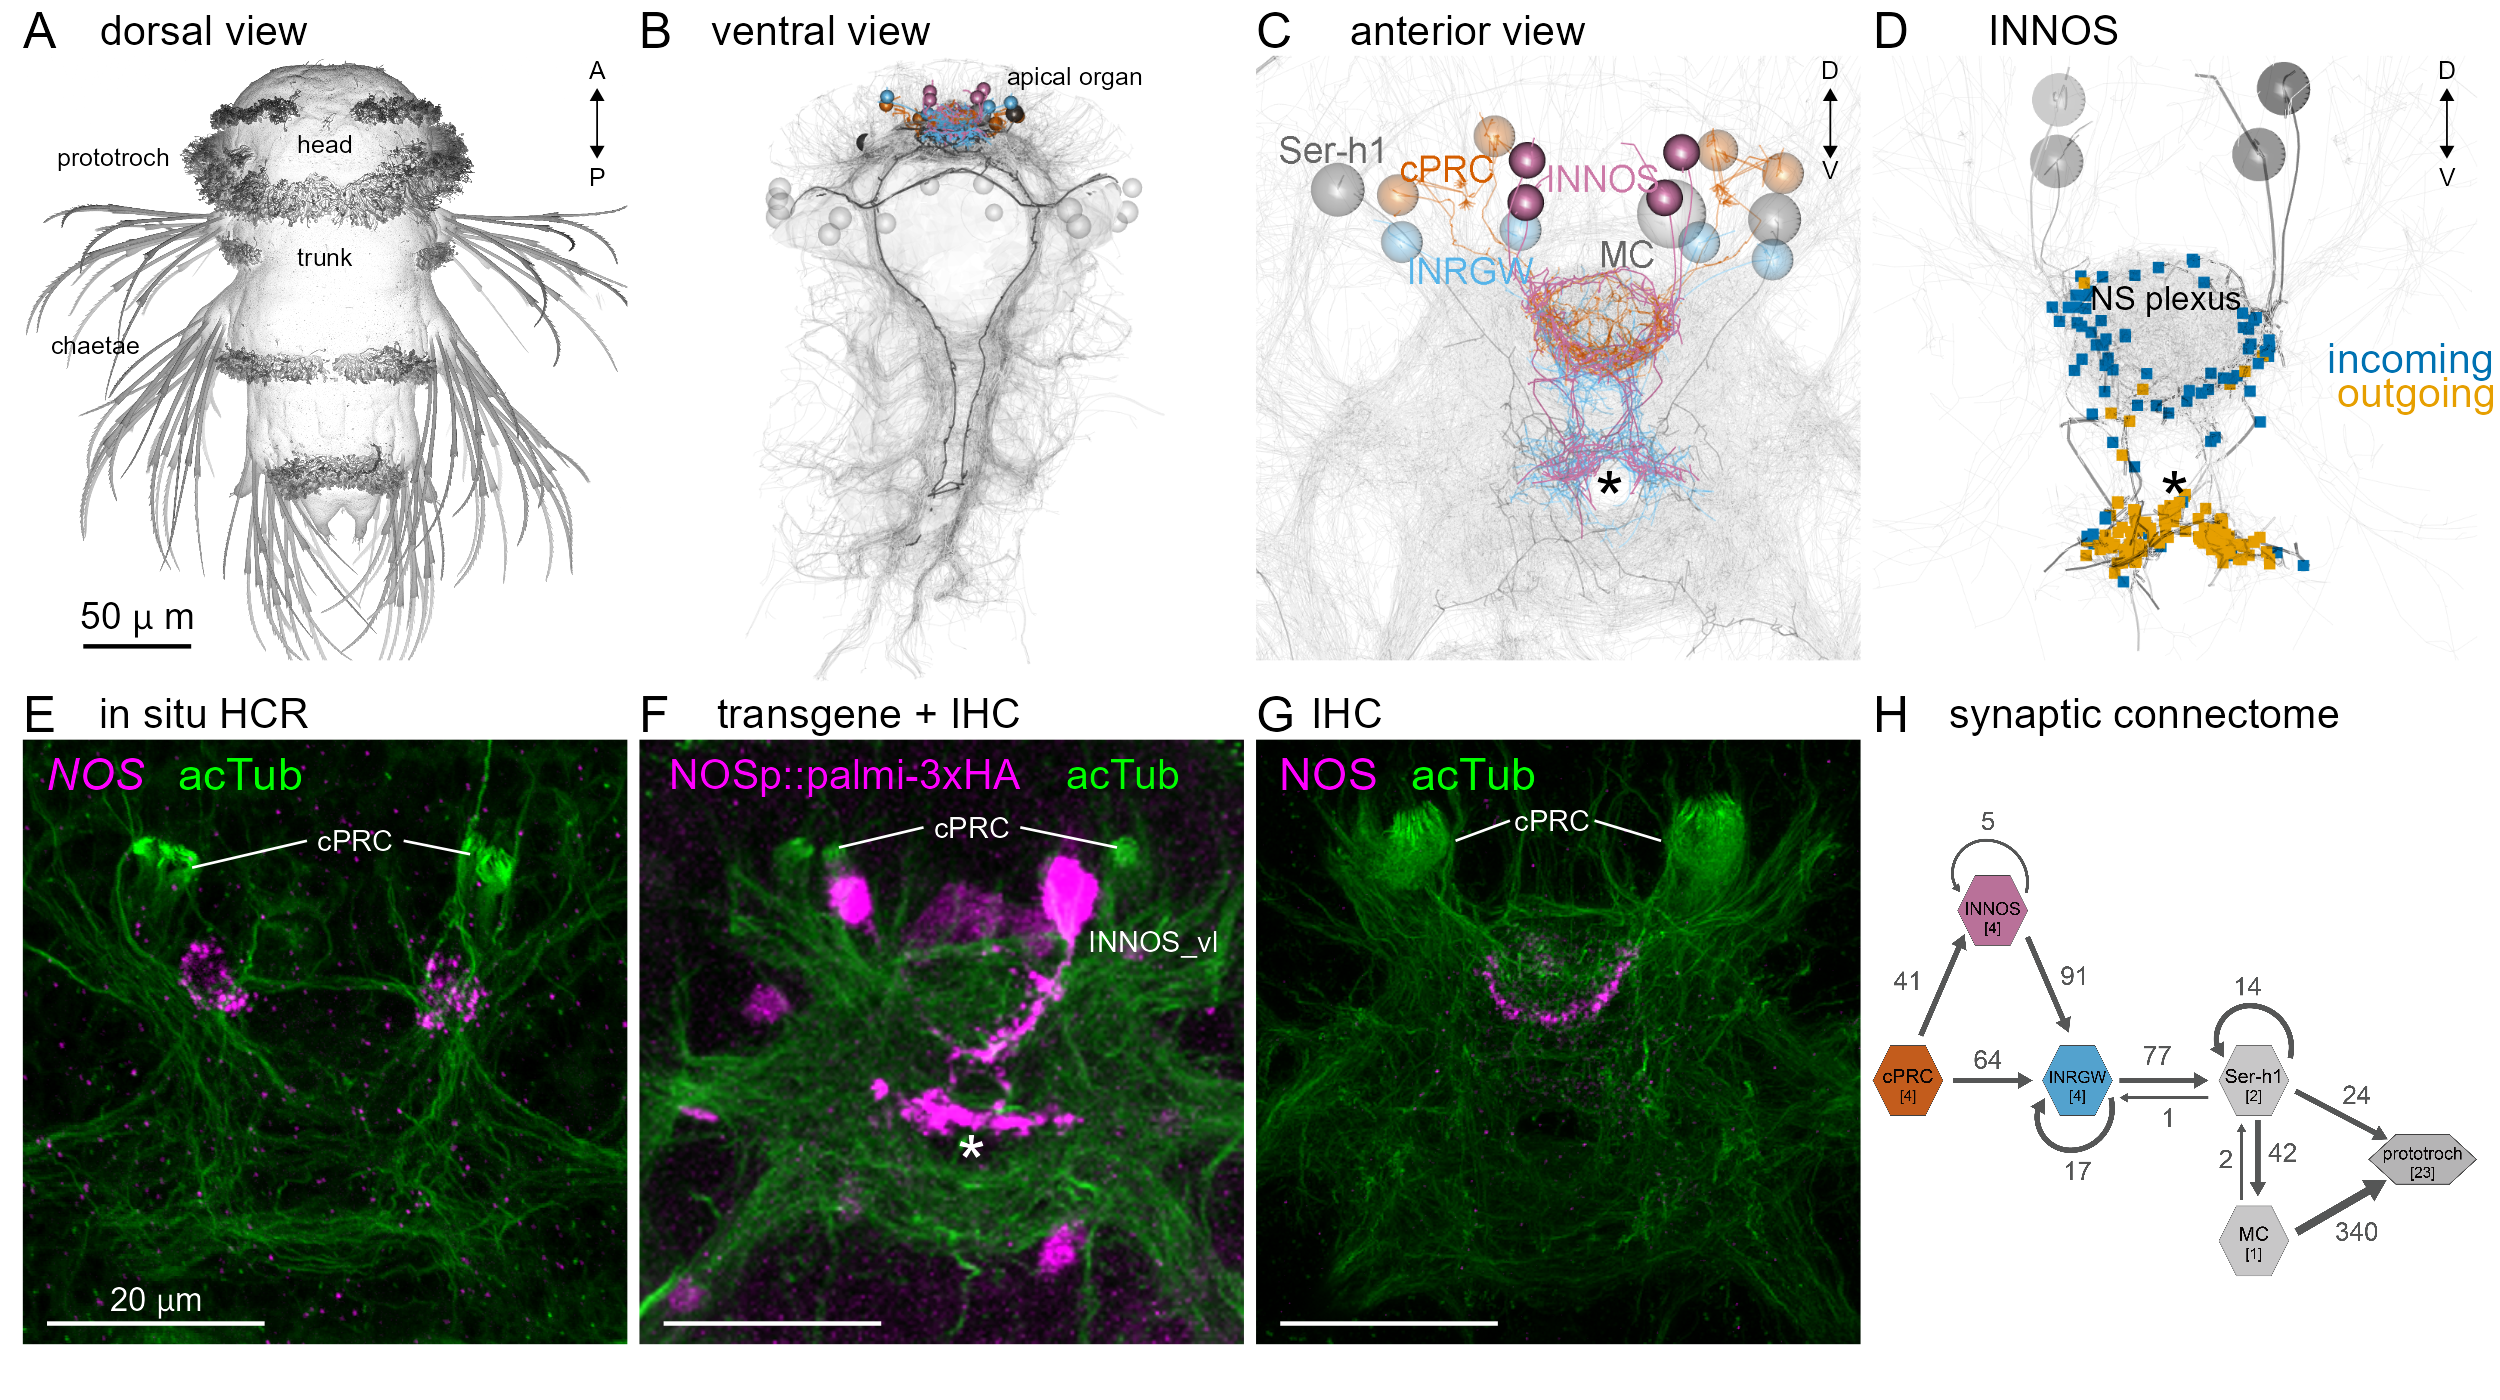
\includegraphics[width=25in]{figures/Fig1} \caption{**Figure 1. Identification of NOS-expressing interneurons (INNOS) within the cPRC circuit.** **(A)** SEM image of a three-day-old Platynereis larva. **(B, C)** Five types of neurons (cPRC, INNOS, INRGW, Ser-h1 and MC) in the cPRC circuit reconstructed in the whole-body transmission electron microscopy (ssTEM) dataset of a three-day-old larva. Ciliated cells labelled with (B) are shown in grey. The INNOS on the ventral side labelled with (C) are shown in purple. Axons and dendrites appear as lines and cell body positions are represented by spheres. **(D)** Expression analysis of the NOS gene (magenta) using in situ HCR. Anterior view of the larva at two-day-old. Co-stained image using acetylated α-tubulin antibody (acTub: green). **(E)** Immunostaining with anti-HA antibody against HA tagged palmitoylated-tdTomato expressed under the upstream of the start site of NOS (NOSp::palmi-3xHA: magenta). Co-staining with acetylated α-tubulin antibody as marker for cilia of cPRC and axonal scaffold (acTub: green). Views of larvae at three-day-old from the anterior side. Insert: One of the reconstructed INNOS is shown from the anterior side. **(F)** Wiring diagram of the cPRC circuit. Hexagons and arrows represent cell groups and their synaptic connections, respectively. Numbers inside hexagons indicate the number of cells grouped in each node. Arrow line thickness (synapse weight) is equal to the number of synapses.}\label{fig:unnamed-chunk-1}
\end{figure}

\textbf{Nitric oxide produced during UV/violet stimulation gates the
output of the cPRC circuit}

The expression of \emph{NOS} in the INNOS interneurons in the cPRC
circuit suggests that NO signalling may be involved in
UV/violet-avoidance. To test this, first we asked whether NO is produced
during UV/violet stimulation of the larvae. We injected the fluorescent
NO-reporter DAF-FM into zygotes and imaged two-day-old larvae while
exposing the ramified sensory cilia of the cPRCs to 405 nm violet light.
Following light stimulation of the cPRCs but not a control area, we
detected an increase in DAF-FM fluorescence in the anterior
neurosecretory neuropil, the region of INNOS projections \textbf{(Figure
2)}.

\begin{figure}
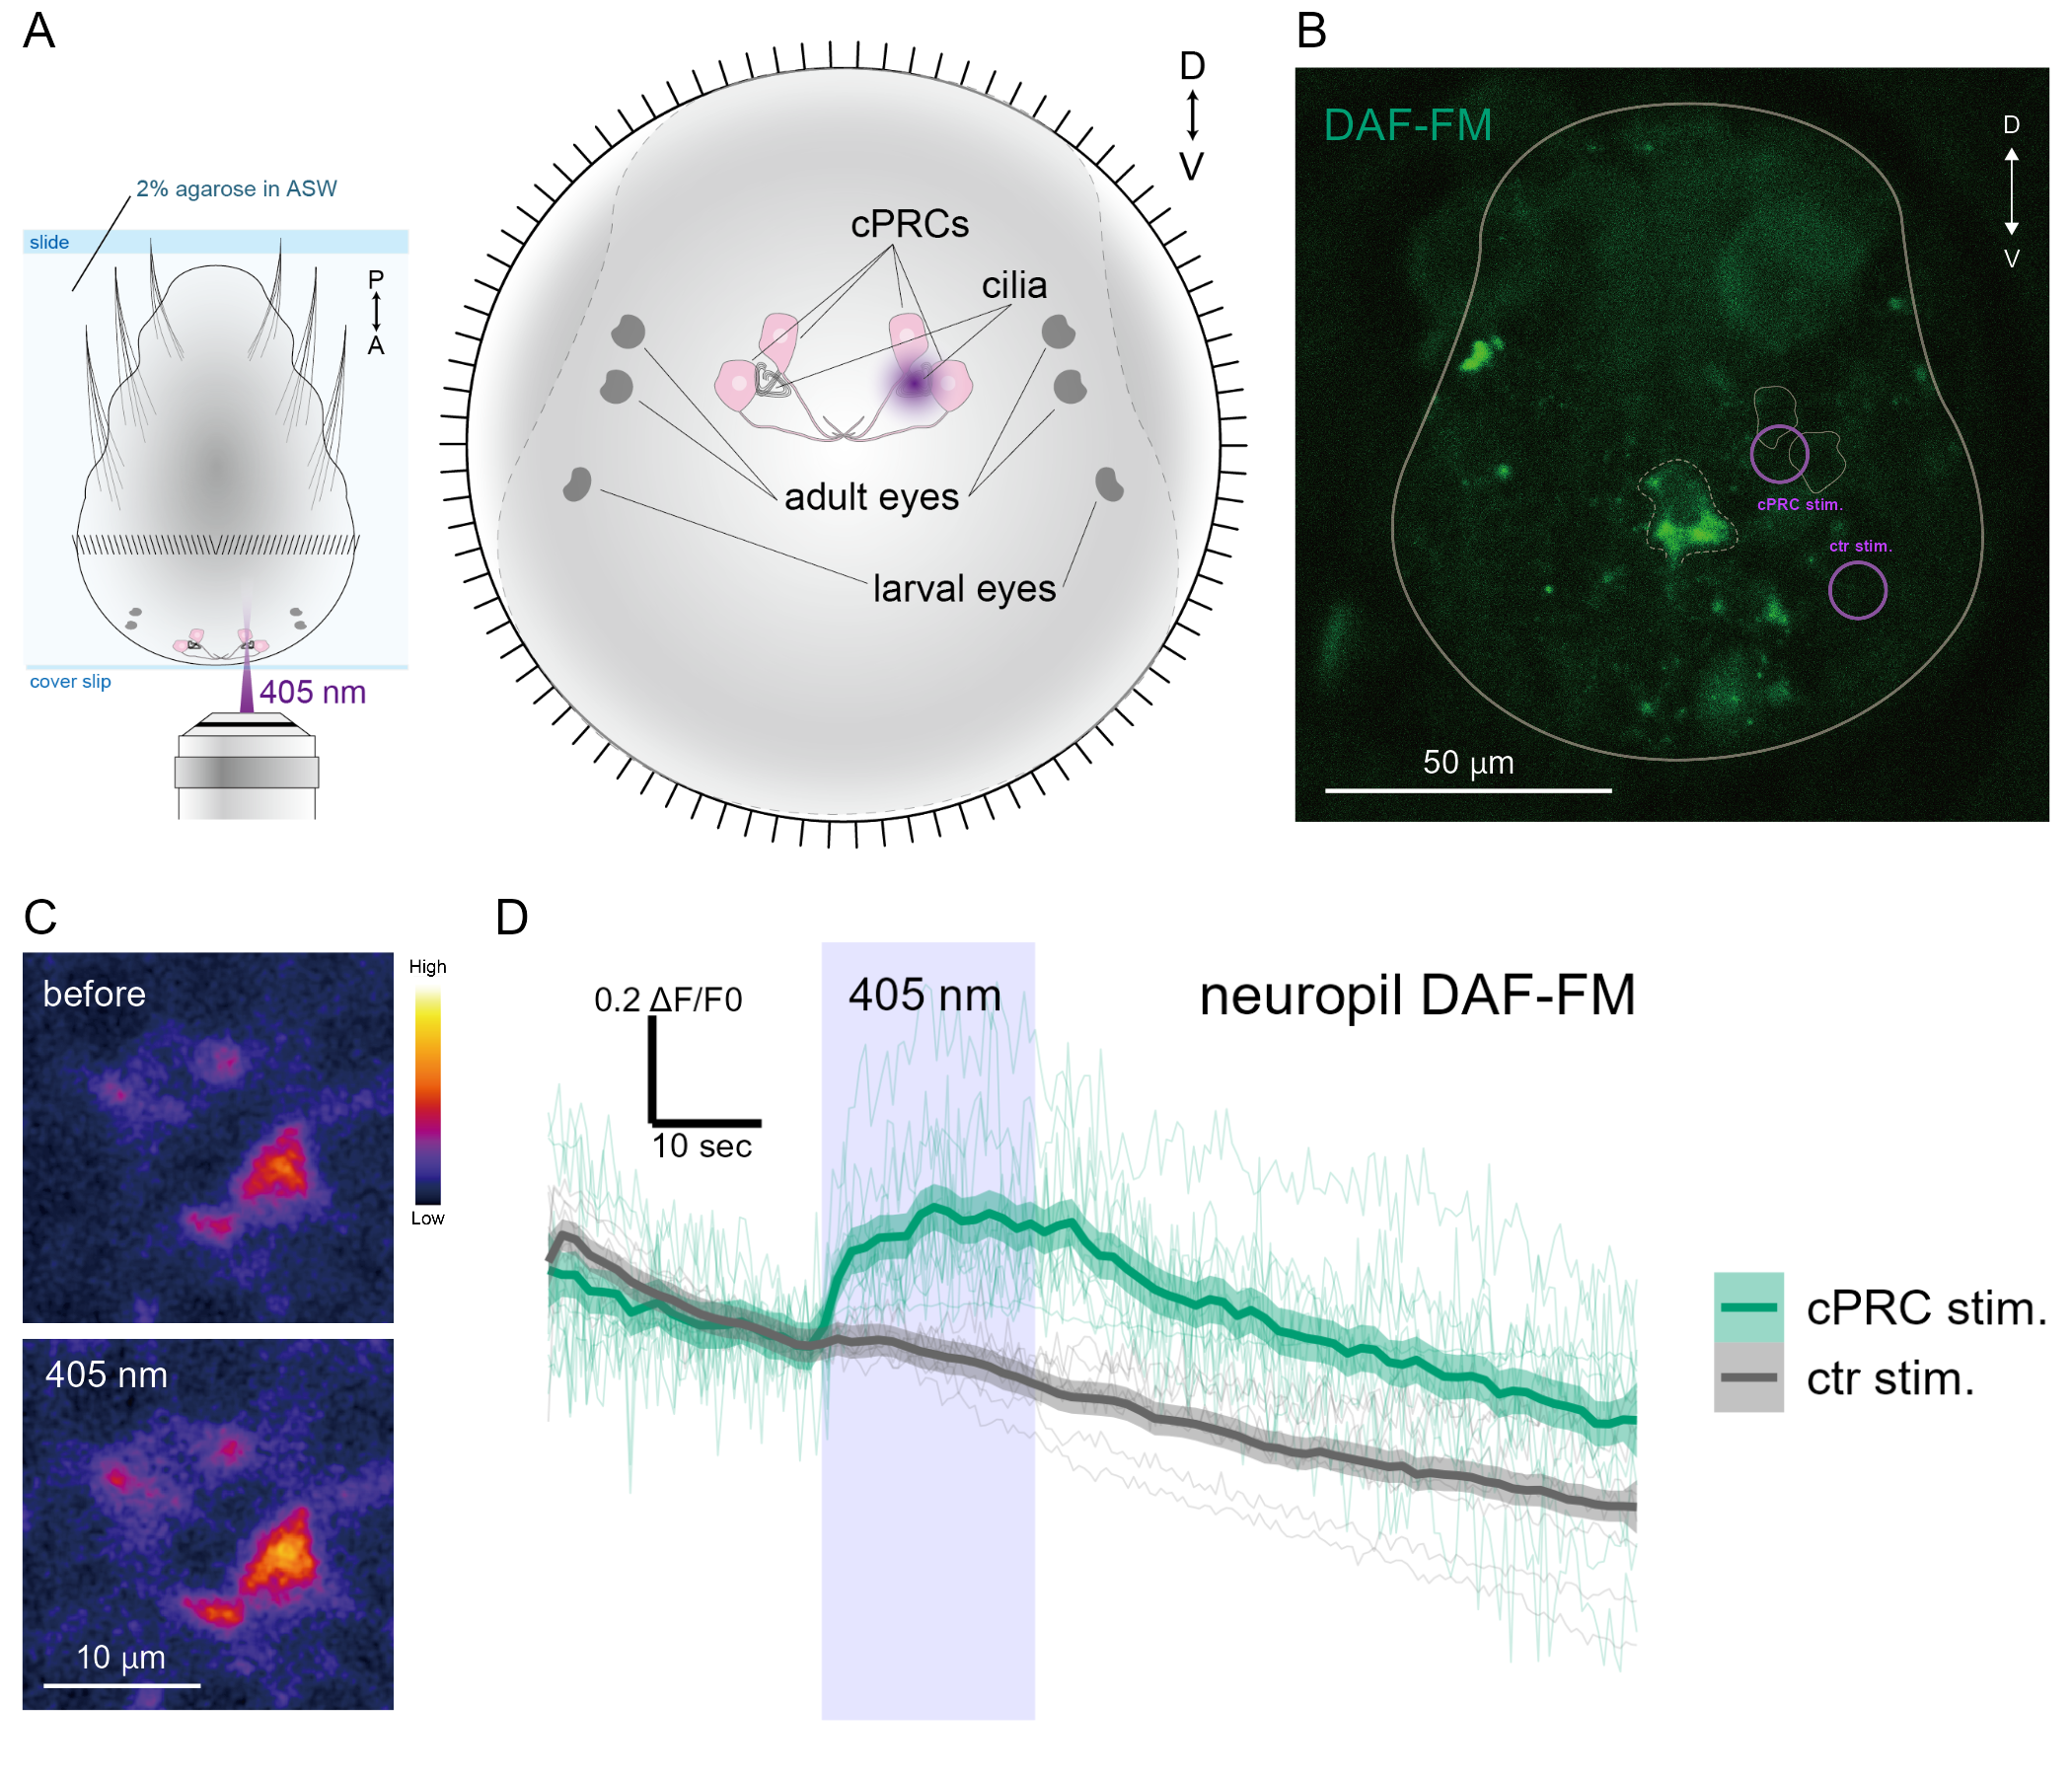
\includegraphics[width=29.17in]{figures/Fig2} \caption{**Figure 2. NO produced by UV/violet stimulation to cPRCs.** **(A)** A NO-positive cell visualised by DAF-FM (green) is shown (dashline). The white line indicates the outer frame of the larva. All subsequent images are of two-day-old larvae. **(B)** Intensity changes before (upper) and during 405 nm light stimulation (lower) in a cell visualised by DAF-FM. **(C)** The intensity of DAF-FM changes over time when cPRC (green) and other cells (ctr: gray) are stimulated with UV/violet (405 nm) light. Purple squares indicate the timing of 405 nm light stimulation, the transparent lines show the optical responses to individual intensities, each intensities are normalized (ΔF/F0) and the dark trace lines and the shaded bands show the mean value and the standard error range of the mean.}\label{fig:unnamed-chunk-2}
\end{figure}

\textbf{Nitric oxide signalling mediates UV-avoidance behaviour}

Next, we wanted to directly test whether NO signalling is involved in
UV/violet avoidance. To achieve this, we generated two
\emph{Platynereis} \emph{NOS} knockout lines with the CRISPR/Cas9
method. We recovered two deletions (NOSΔ11/Δ11 and Δ23/Δ23), both
leading to frame-shift and an early stop codon and thus likely
representing null alleles \textbf{(Figure 3A)}. We could establish a
homozygous line for both mutations indicating that NOS is not an
essential gene. To quantify UV avoidance, we recorded the trajectories
of freely swimming wild type and mutant larvae in vertical columns,
illuminated laterally from two opposite sides with 395 nm UV light
\textbf{(Figure 3B, C and Figure 3---figure supplement 1A-D)}. As
previously shown, wild-type larvae swim downward following
non-directional UV/violet light stimulation (Verasztó et al., 2018). In
contrast, both two- and three-day-old homozygous \emph{NOS}-mutant
larvae showed a strongly diminished UV-avoidance response
\textbf{(Figure 3B-D and Figure 3---figure supplement 1)}. This
phenotype is similar to the defective UV-avoidance of \emph{c-opsin1}
mutant larvae and reveals a requirement for NOS in UV-avoidance
behaviour (Verasztó et al., 2018). Wild type but not mutant larvae also
showed an increase in swimming speed under UV light that may be due to
downward swimming trajectories (swimming with gravity) \textbf{(Figure
3---figure supplement 1C,D)}. We also tested directional phototaxis, by
exposing larvae to 480 nm directional and collimated light from the top
of the column. Three-day-old but not two-day-old \emph{NOS}-mutant
larvae also showed reduced phototactic behaviour, suggesting a function
for \emph{NOS} in the visual eyes that mediate three-day-old phototaxis
(Randel et al., 2014) \textbf{(Figure 1---figure supplement 1A,B)}. To
distinguish between an acute or developmental function of NOS in light
responses, we next tested larvae exposed to the NOS inhibitor L-NAME.
Larvae incubated for 5 min in 0.1 mM or 1 mM L-NAME showed a
dose-dependent inhibition of UV avoidance. In contrast, phototaxis was
not effected \textbf{(Figure 3E)}. Overall, our results indicate an
acute requirement for NOS signalling in UV-avoidance and a possible
indirect, developmental role in visual phototaxis.

\begin{figure}
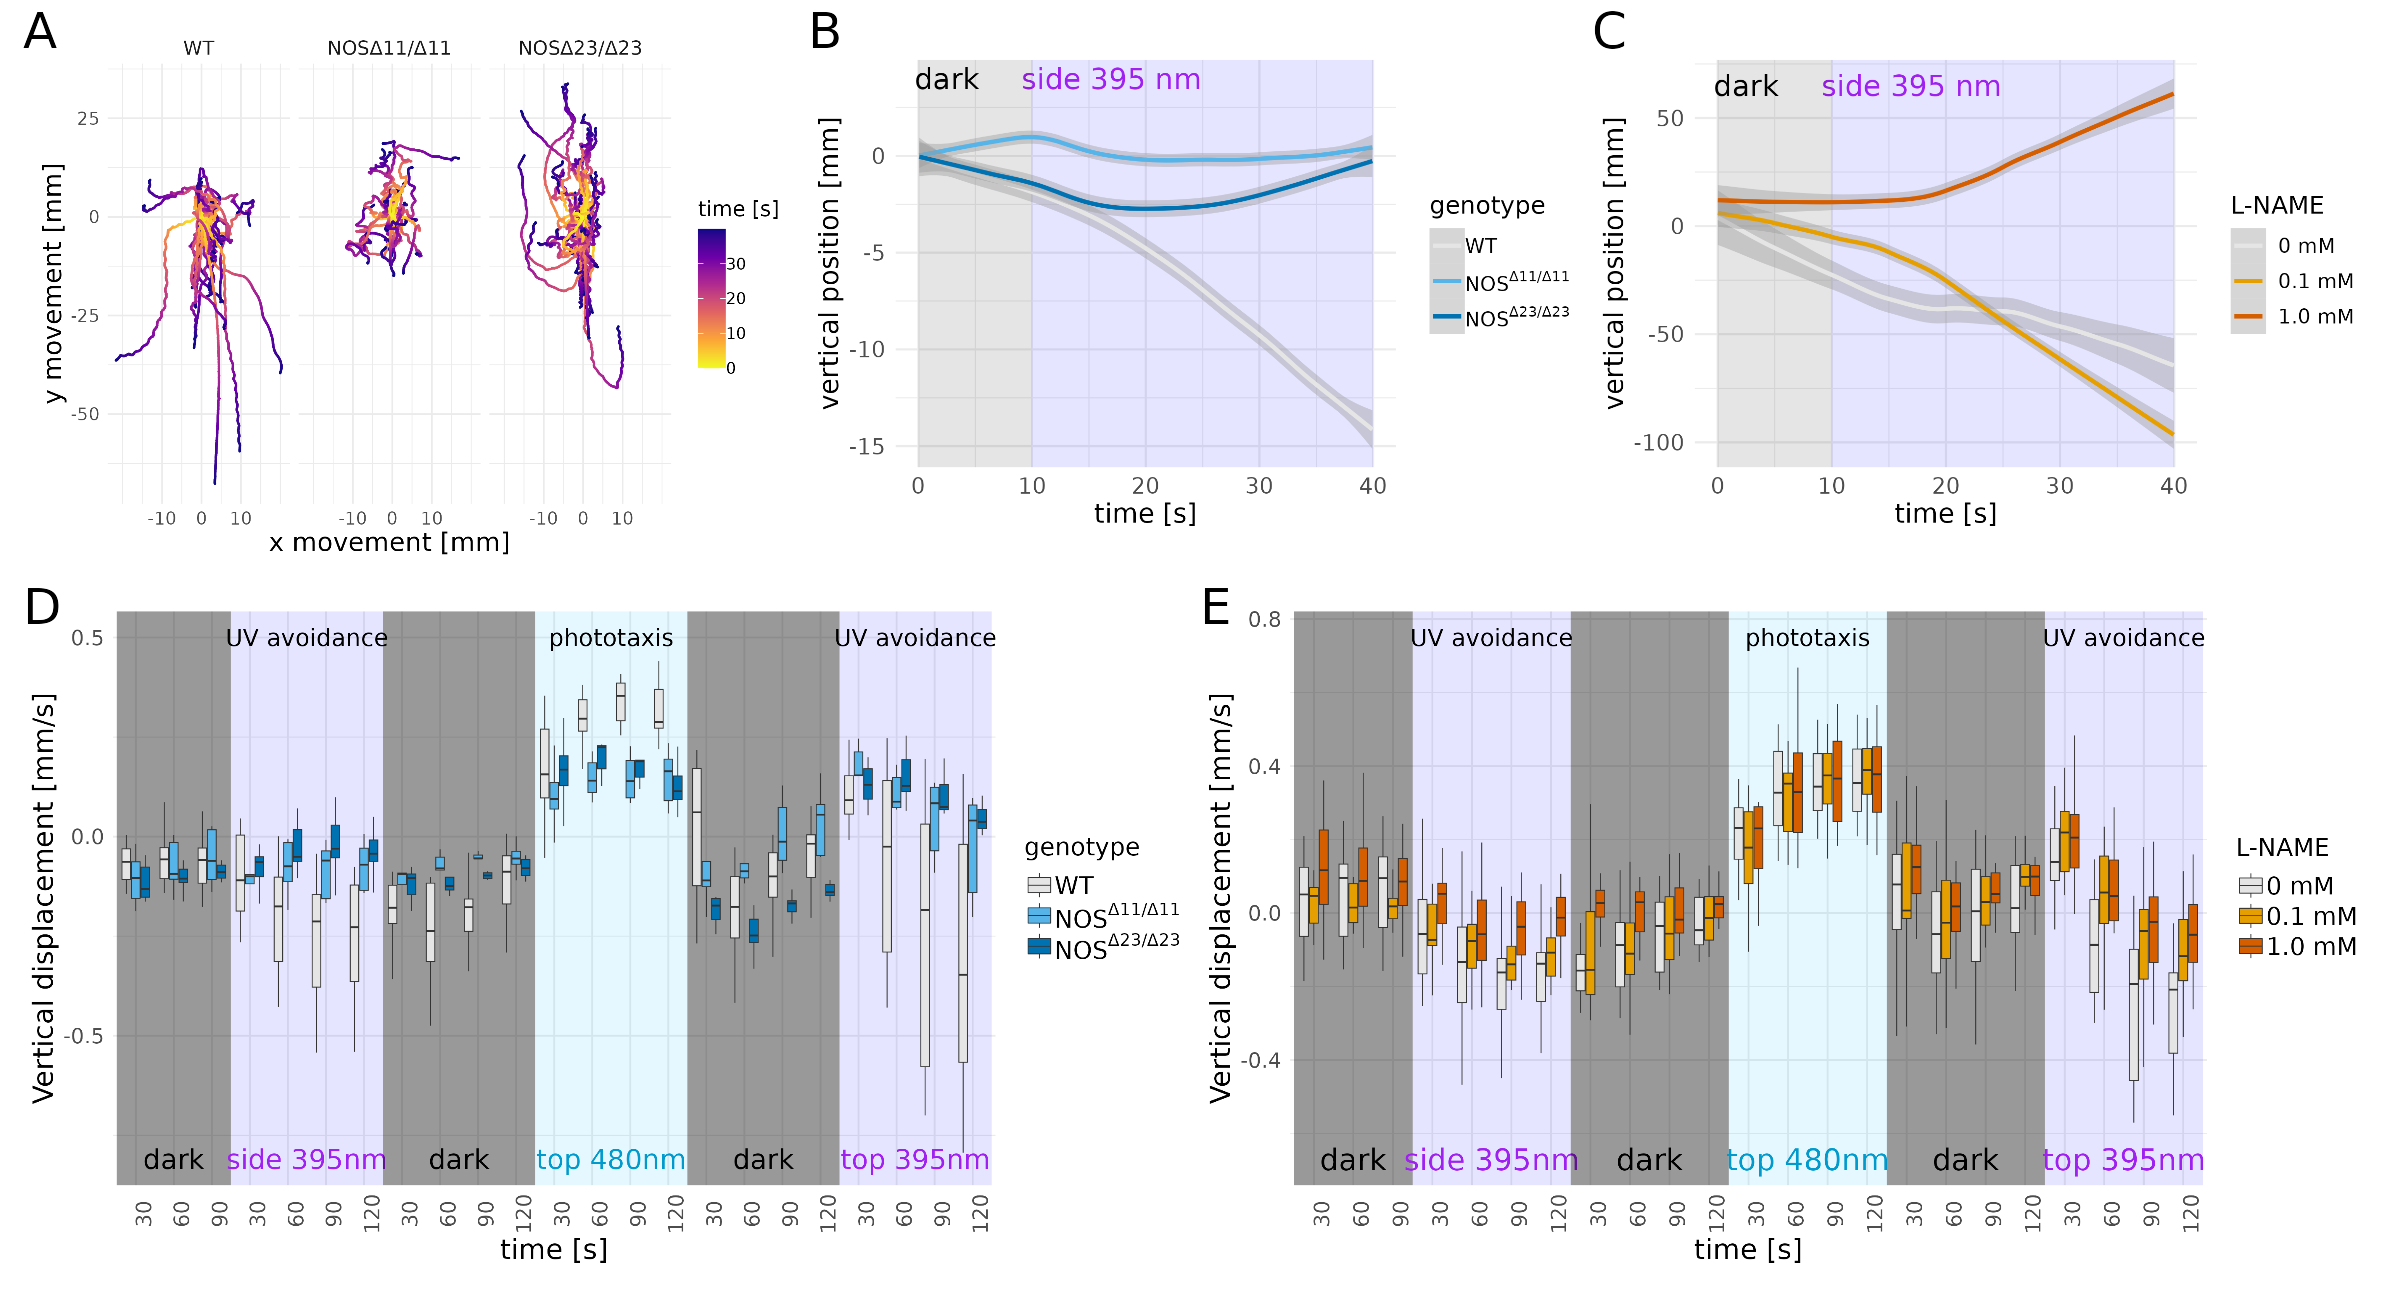
\includegraphics[width=33.33in]{figures/Fig3} \caption{**Figure 3. Larvae with inhibited NOS have a delayed response to UV-avoidance.** **(A)** Top: The domain and Exon/Intron structure of NOS. Bottom: Close-up region showing the genomic locus of NOS gene and the wild-type sequence (WT) targeted by CRISPR/Cas9. The generated mutants (NOSΔ11, NOSΔ23) are also shown. Pink indicates target sites. Gray shows PAM sequences, red shows stop codons. **(B)** Overlaid trajectories for WT (n=32) and NOS mutant (NOSΔ11/Δ11, n=26 and NOSΔ23/Δ23, n=47) at three-day-old larvae. 0 sec as the starting point. After 10 sec, UV (395 nm) stimulation from the side. **(C)** The temporal changes in the vertical position of the WT and mutant larvae before (dark) and after UV stimulation (side 395 nm) are shown. The starting points of each larval trajectory are set to 0. **(D)** Vertical swimming in wild-type (WT) and mutant (NOSΔ11 and NOSΔ23) larvae at three-day-old stimulated with UV (395 nm) light from side, blue (488 nm) light from top and UV (395 nm) light from top. The data are shown in 30 s bins. **(E)** Vertical swimming in larvae treated with NOS inhibitors, L-NAME at three-day-old stimulated with UV (395 nm) light from side, blue (488 nm) light from top and UV (395 nm) light from top. The data are shown in 30 s bins.}\label{fig:unnamed-chunk-3}
\end{figure}

\textbf{NO feedback tunes cPRC responses to UV/violet stimulation}

To investigate how NO signalling alters the dynamics of the cPRC
circuit, we carried out calcium imaging experiments. We ubiquitously
expressed the calcium sensor GCaMP6s in larvae and imaged calcium
signals during 405 nm stimulation of the cPRCs. As we have shown
previously, a 20-sec local stimulation of cPRC cilia lead to a transient
increase in cPRC calcium levels, followed by a transient decrease
(Verasztó et al., 2018). After \textasciitilde20-sec, calcium levels in
cPRCs were raising again, reaching higher levels than at the start of
the stimulus -- a response that may involve depolarisation. This
activation phase occurs after the 20 sec stimulation period and is
likely due to a delayed neuroendocrine feedback (Verasztó et al., 2018).
To determine whether NO mediates such a feedback, we repeated the
experiment in \emph{NOS}-mutant larvae. While we detected the initial
activation phase followed by inhibition, in \emph{NOS}-mutants this was
not followed by delayed activation and calcium levels dropped to a low
steady-state level \textbf{(Figure 4E,F)}. We thus identified a
requirement for NO signalling in the late-phase activation of cPRCs.

\textbf{Two unconventional guanylyl cyclases are expressed in the cPRCs}

Next, we aimed to identify the NO-receptor in the cPRCs. NO generally
acts via soluble guanylate cyclases (sGC), belonging to the guanylate
cyclase family with a CYC domain (PFAM domain: PF00211). NO binding to
the heme group of sGC leads to increased cyclic guanosine monophosphate
(cGMP) production. Analysis of sGCs in \emph{Platynereis} indicated that
these genes are not expressed in any of the cells of the cPRC circuit
(Verasztó et al., 2017). Recently, Moroz and coworkers reported an
atypical but widely conserved family of guanylyl cyclases with a NIT
(nitrite/nitrate sensing) domain (PF08376) (NIT-GC) as potential
mediators of NO signalling (Moroz et al., 2020). To search for NIT-GCs
in \emph{Platynereis}, we searched transcriptome resources and retrieved
15 potential NIT-GC homologs \textbf{(Figure 4---figure supplement 1)}.
To analyse the relationship of these sequences to metazoan NIT-GCs, we
retrieved protein sequences with a CYC domain from the transcriptome and
genome databases of 45 metazoan species and 2 choanoflagellate species.
We carried out cluster analysis and did phylogenetic reconstruction on a
group of membrane-bound guanylyl cyclases with sGCs as an outgroup. In
agreement with Moroz et al. (Moroz et al., 2020), we found a group of
GCs with NIT domains with representatives in placozoans, cnidarians,
some ecdysozoans, echinoderms, and lophotrochozoans. The 15
\emph{Platynereis} sequences were parts of several major and ancient
clades of the tree \textbf{(Figure 4---figure supplement 1)}. To
characterise the expression of NIT-GCs, we used previously published
spatially mapped single-cell transcriptome data (Achim et al., 2015;
Williams et al., 2017). Among the 15 NIT-GCs, two showed high and
specific expression in the cPRCs and one was expressed in the INNOS
cells \textbf{(Figure 4---figure supplement 1)}. In the single-cell
data, we could identify the cPRCs by the specific expression of c-opsin1
and a pedal-peptide2 neuropeptide precursor (MLD proneuropeptide)
(Arendt et al., 2004; Williams et al., 2017), which have previously been
described as cPRC markers \textbf{(Figure 4---figure supplement 2A)}.
The INNOS cells were identified by NOS expression and spatial mapping in
the brain (Achim et al., 2015). We decided to focus on two NIT-GCs
expressed in the cPRCs and with a full-length sequence, NIT-GC1 and
NIT-GC2. To confirm the single-cell data, we first carried out in situ
HCR with probes for \emph{NIT-GC1} and \emph{NIT-GC2} mRNA. Both genes
were specifically expression in the four cPRCs, as confirmed by
co-labeling with an acetylated α-tubulin antibody and with an HCR probe
against \emph{pedal peptide 2/MLD proneuropeptide} \textbf{(Figure 4A,B
and Figure 4---figure supplement 2A-C)}. To analyse the subcellular
localisation of NIT-GC1 and NIT-GC2 at the protein level, we raised and
affinity-purified polyclonal antibodies against a specific peptide
sequence from both proteins. In immunostainings, we found that NIT-GC1
was localise to the region corresponding to the axonal projections of
the cPRCs in the anterior nerve plexus \textbf{(Figure 4C)}.
Co-immunostaining with the rabbit NIT-GC1 antibody and a custom rat
antibody raised against a fragment of \emph{Platynereis} NOS, revealed
that both proteins were localised in close proximity in the
neurosecretory plexus \textbf{(Figure 4---figure supplement 2D)}. In
contrast, NIT-GC2 specifically labelled the large sensory ciliary region
of the cPRCs \textbf{(Figure 4D)}. These different subcellular
localisations suggest that the two NIT-GCs are involved in different
intracellular signalling processes in the ciliary and axonal regions of
the cPRCs.

\textbf{NIT-GC1 produces cGMP in an NO-dependent manner}

To further characterise these atypical guanylyl cyclases, we focused on
NIT-GC1 and carried out in vitro experiments. In bacteria, NIT domains
are thought to regulate cellular functions in response to intra- or
extracellular nitrate and nitrite. NIT-GC1 has a NIT domain and a highly
conserved cyclase domain that is expected to catalyse cGMP synthesis
\textbf{(Figure 4I)}. The NIT domain may render NIT-GC1 dependent on NO
signals. To test this, we co-expressed the synthetic cGMP indicator
Green cGull (Matsuda et al., 2016) and NIT-GC1 in cultured cells COS-7
(monkey kidney). For balanced expression, we used a single plasmid with
the two open-reading frames separated by the 2A self-cleaving peptide
\textbf{(Figure 4J)}. Application of the NO donor SNAP lead to increased
cGMP levels, an effect we did not observe when cells were exposed to
DMSO or when Green cGull was expressed alone \textbf{(Figure 4K-M)}. To
test whether cGMP production is dependent on the NIT domain, we also
tested a deletion construct of NIT-GC1 lacking the NIT domain
\textbf{(Figure 4I)}. Cells expressing this construct and Green cGull
did not show increased cGMP levels when exposed to SNAP \textbf{(Figure
4N)}. These results indicate that NIT-GC1 is able to catalyse cGMP
production in an NO-dependent manner and this function requires the NIT
domain. These results establish NIT-GC1 as a biochemical NO sensor.

\textbf{NIT-GC1 is required for NO-mediated feedback to cPRCs during the
UV response}

To test the in vivo function of NIT-GC1 and NIT-GC2 in cPRC responses,
we combined calcium imaging with morpholino-mediated knockdowns. We used
two translation-blocking morpholinos for each \emph{NIT-GC} gene and
tested knockdown efficiency by immunostaining injected animals with the
NIT-GC1 and NIT-GC2 antibodies \textbf{(Figure 4---figure supplement
2E,F)}. For both genes, the morpholinos led to a strong reduction in the
respective antibody signal, confirming efficient knockdown and antibody
specificity.

In NIT-GC1 morphant larvae, the delayed activation of cPRCs following
405 nm stimulation did not occur \textbf{(Figure 4G)}. This phenotype is
similar to the phenotype of \emph{NOS} mutants suggesting that NIT-GC1
acts as the NO sensor in cPRCs to drive their delayed activation. This
could occur via increased cGMP production and the opening of a
cyclic-nucleotide-gated (CNG) channel specific to cPRCs. NIT-GC2
morphant larvae, in contrast, showed a step-up increase in calcium
following light stimulation \textbf{(Figure 4H)}. The calcium signal
decayed during stimulation and was off after light off. These data
support an essential role for ciliary-localised NIT-GC2 in suppressing
cPRC calcium following its transient rise at stimulus onset. Overall,
these knockdown experiments revealed different signalling mechanisms for
the two NIT-GCs that may be due to their different subcellular
localisations.

\begin{figure}

\includegraphics[width=38.89in]{figures/Fig4} \caption{**Figure 4. cPRC-specific expression of NIT-GC1 localises in close proximity to NOS in the ANS region.** **(A, B)** Expression analysis of the NIT-GC1 (C) and NIT-GC2 (D) gene (magenta) using in situ HCR. Co-staining image using acetylated α-tubulin antibody (ac α-tub: green). **(C, D)** Localisation analysis using NIT-GC1 and NIT-GC2 antibodies. Green shows co-staining with acetylated α-tubulin antibody (ac α-tub). **(E, F)** Changes over time in GCaMP6s intensities in cPRC when stimulated with UV in WT (dark yellow) and NOS mutant (E: NOSΔ11/Δ11, F: NOSΔ23/Δ23) (light pink) larvae. **(G, H)** Changes over time in GCaMP6s intensities in cPRC when stimulated with UV in NIT-GC1 (G: NIT1) and NIT-GC2 (H: NIT2) knockdown by morpholino (MO1 and 2) larvae. **(I)** The domain structure of NIT-GC1. Below shows the mutant NIT-GC1 (ΔNIT-GC1) with deletion of the NIT domain. Grey squares indicate the transmembrane region (TM). **(J)** A schematic of the NIT-GC1 assay; COS7 cells were used to express NIT-GC1 and the cGMP indicator Green cGull, and the NO donor SNAP and DMSO as control. Green cGull shows cGMP-dependent green fluorescence. **(K-N)** The intensity changes in cGMP fluorescence over time for the four conditions are shown. Gray traces show the optical responses to individual intensities (n > 6). The individual intensities are normalized (ΔF/F0). The dark line shows the mean value and the band the standard error range of the mean. The respective solution was acted on 2 min after the start of imaging (grey bars).}\label{fig:unnamed-chunk-4}
\end{figure}

\textbf{NO signalling shapes the dynamics of the cPRC circuit}

To investigate how NO and NIT-GC signalling influence the dynamics of
the cPRC circuit, we imaged calcium signals from postsynaptic neurons in
wild type, mutant and morphant larvae. We were able to image the
activity of all neurons in the cPRC circuit (INNOS, INRGW, Ser-h1 and
MC). The MC cell was identified based on its position and intrinsic
activity. To unambiguously identify all other cells from which we
recorded calcium signals, we developed an on-slide immunostaining method
\textbf{(Figure 5---figure supplement 1)}. We used the cell-specific
antibody markers against RYamide (INNOS), RGWamide (INRGW) and serotonin
(Ser-h1) (Conzelmann et al., 2011) to immunostain agar-embedded larvae
following calcium imaging. Based on the position of the nuclei, we could
correlate live and fixed samples at a single-cell precision
\textbf{(Figure 5A,B)}. Due to the stereotypy of the larvae, we could
also identify neurons based on their position and activity in
activity-correlation maps \textbf{(Figure 5C)}.

We first quantified the responses of the INNOS and INRGW interneurons
during 405 nm stimulation of the cPRCs. In both wild type and
\emph{NOS}-mutant larvae, INNOS cells showed an increase in calcium
during stimulation \textbf{(Figure 5D)}. This response was suppressed in
NIT-GC2 morphant larvae \textbf{(Figure 5E)} revealing an essential role
for NIT-GC2-mediated cPRC suppression in INNOS activation. In contrast,
INRGW cells were initially inhibited, followed by a delayed activation
paralleling the second activation phase of cPRCs. This late INRGW
response was lacking in \emph{NOS}-mutants \textbf{(Figure 5F,G)}. In
NIT-GC2 morphants, INRGW cells showed a transient increase in calcium
that decayed after light off and a delayed activation was not present.
Next, we imaged calcium signals from Ser-h1 and MC neurons in wild type
and \emph{NOS} mutant larvae. Ser-h1 cells showed an activation profile
that correlated with cPRC activity, including a reduction in calcium
during stimulation followed by rebound, a response that was defective in
\emph{NOS} mutants. MC cells showed sustained activation, including a
late-phase that was lacking in \emph{NOS} mutants \textbf{(Figure
5H,I)}. These data suggest that during 405 stimulation the Ser-h1 cells
are inhibited and MC cells are activated, and this regulation is
NO-dependent. This pattern is expected to inhibit ciliary activity in
the prototroch but not in the other ciliary bands, triggering
NO-dependent downward swimming.

\begin{figure}
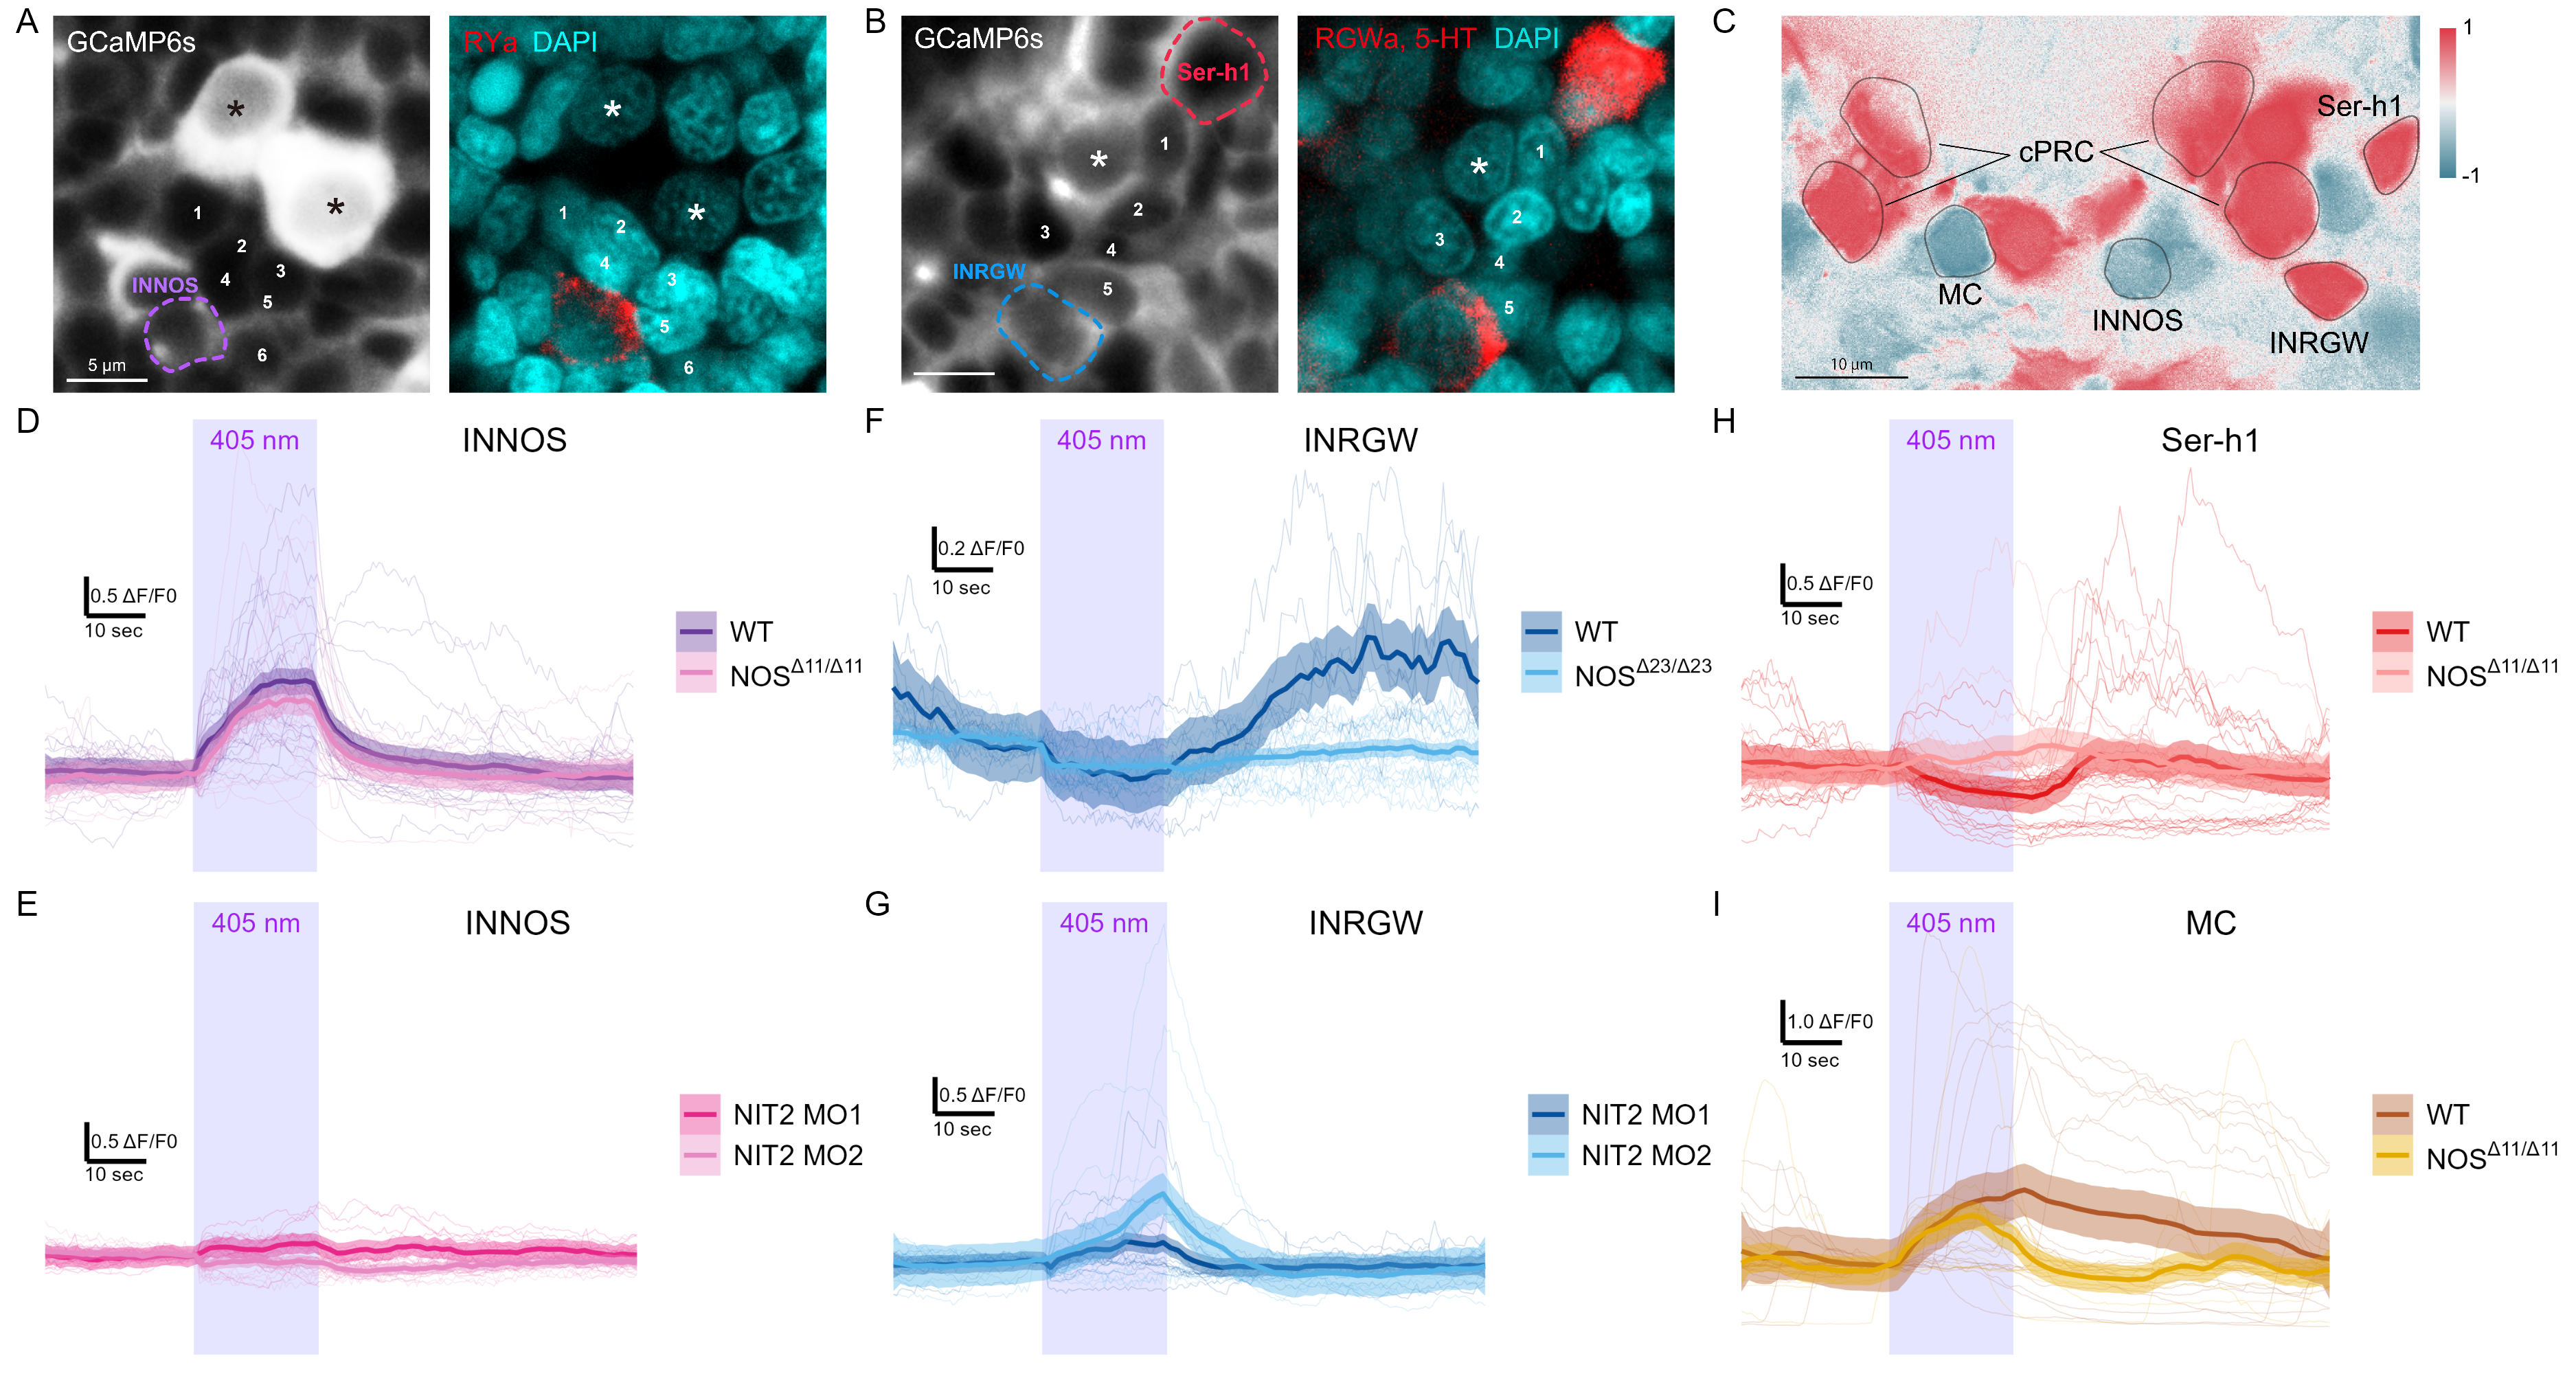
\includegraphics[width=52.08in]{figures/Fig5} \caption{**Figure 5. NO produced by UV stimulation to cPRCs induces a depolarising response in cPRC via NIT-GC1.** **(A, B)** Each left figure shows a calcium imaging using GCaMP6s. The respective right figures show immunostaining images of the same positions in the respective left figures, (A) shows RYamide antibodies, (B) shows RGWamide and serotonin (5-HT) antibodies in red and DAPI in cyan. Asterisks indicate the nuclei of the cPRC, respectively, and the nuclei of the cells that were identified from the arrangement of the surrounding cells are indicated by numbers. From the position of the cells, the calcium imaging data identify INNOS in (A) and INRGW and Ser-h1 in (B), respectively. **(C)** Correlation (Pearson's r) map of neuronal activity of the INNOS, INRGW, Ser-h1 and MC neurons. **(D)** Changes over time in GCaMP6s intensities in INNOS when cPRC is stimulated with UV in WT (dark purple) and NOSΔ11/Δ11 mutant (light purple) larvae. **(E)** Changes over time in GCaMP6s intensities in INNOS when cPRC is stimulated with UV in NIT-GC2 morphants (MO1 and MO2: pink and light pink) larvae. **(F)** Changes over time in GCaMP6s intensities in INRGW when cPRC is stimulated with UV in WT (dark blue) and NOSΔ23/Δ23 mutant (light blue) larvae. **(G)** Changes over time in GCaMP6s intensities in INRGW when cPRC is stimulated with UV in NIT-GC2 morphants (MO1 and MO2: blue and light blue). **(H, I)** Changes over time in GCaMP6s intensities in Ser-h1 and MC when cPRC is stimulated with UV in WT (Ser-h1 and MC: dark red and brown) and NOSΔ11/Δ11 mutant (Ser-h1 and MC: light red and brown) larvae.}\label{fig:unnamed-chunk-5}
\end{figure}

\textbf{Mathematical modelling of cPRC-circuit dynamics}

{[}to be added{]}

\begin{figure}
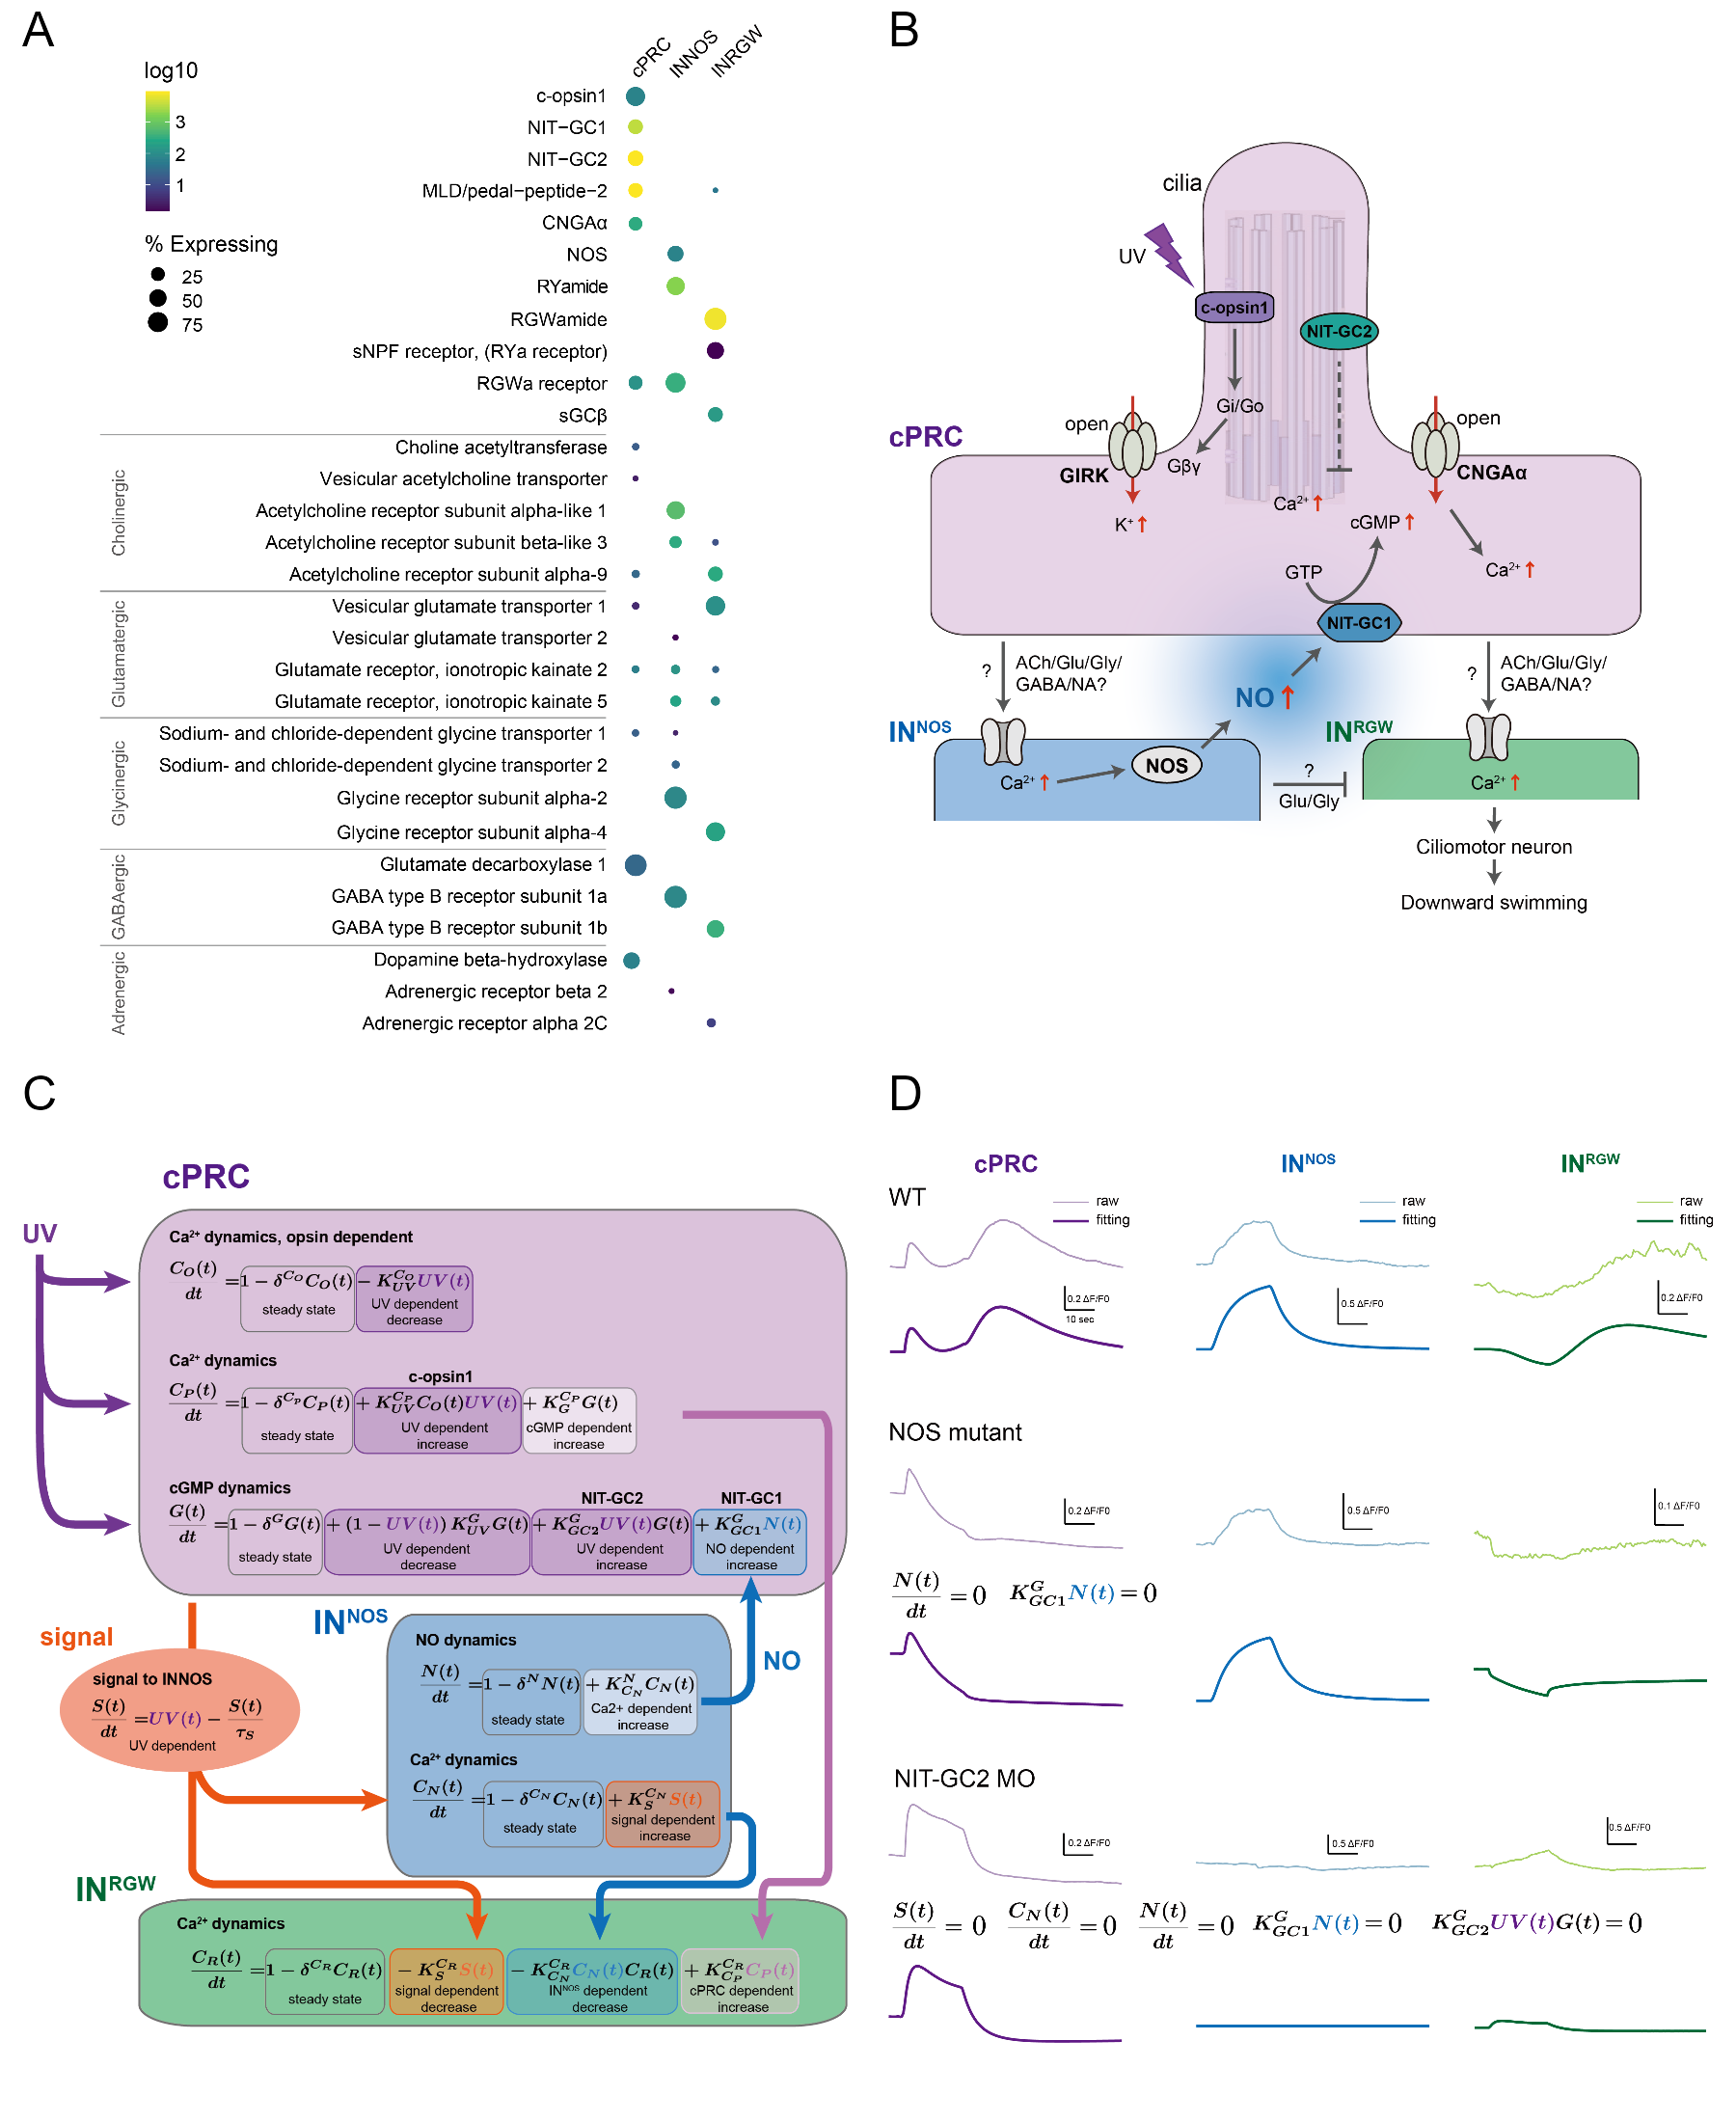
\includegraphics[width=25in]{figures/Fig6} \caption{**Figure 6. Gene expressions and signalling mechanisms between cPRC, INNOS and INRGWa.** **(C)** Dot plot of genes (columns) expressed in three types of cells (rows) in the cPRC circuit using single cell RNA-Seq. The size of the dots is expressed in proportion to the percentage of cells expressing that gene relative to all cells. The colours represent the normal logarithm of the number of transcripts in the cells expressing the gene. **(D)** Schematic diagram of the signalling pathway of the cPRC circuit, focusing on the NO feedback.}\label{fig:unnamed-chunk-6}
\end{figure}

\hypertarget{discussion}{%
\subsection{Discussion}\label{discussion}}

The activity of synaptic circuits is richly modulated monoamines,
neuropeptides and gaseous molecules. Our work revealed an essential role
for NO-mediated signalling in driving UV/violet avoidance behaviour. NO,
produced by postsynaptic interneurons, feeds back to their presynaptic
photoreceptor partners leading to their delayed activation. This
late-phase activation of cPRCs drives circuit output through projection
interneurons and ciliomotor neurons. In the cPRC circuit, synaptic
connectivity alone is not sufficient to drive circuit dynamics and
behavioural change.

We identified cPRC-expressed NIT-GC1 as a new type of NO sensor. NIT-GC1
is localised to the axonal projections of the cPRCs in the anterior
neurosecretory plexus of the brain. Here, cPRC axons intermingle and
synapse on INNOS neurites that contain NOS. NO-mediated feedback
signalling thus likely occurs in the neurosecretory plexus where NOS-
and NIT-GC1-containing projections are in close proximity and where we
could detect NO production following UV stimulation.

We showed that NIT-GC1 can produce cGMP in a NO-dependent manner. In
cPRCs, increased cGMP levels could open CNGAα, a cyclic nucleotide-gated
channels specifically expressed in cPRC (Tosches et al., 2014), leading
to cPRC delayed depolarisation, even after UV off.

NO is a free radical with a half-life of 5 msec in vivo and a signalling
range limited to a few tens of nanometers. In neuronal signalling, NOS
and sGC have been found to localise at close proximity at synapses
{[}Burette et al. (2002){]}(Garthwaite, 2015). We identified 12 sGCs in
\emph{Platynereis}, but none of these is expressed in the cPRC. Instead,
we identified an unconventional NIT-domain containing GC, NIT-GC1 as the
mediator of NO retrograde signalling. The NIT domain was first
identified in bacteria and animal NIT-GCs have only been recently
reported (Moroz et al., 2020; Shu et al., 2003). Bacterial NIT domains
regulate cellular functions in response to changes in extracellular and
intracellular nitrate and/or nitrite concentrations (Camargo et al.,
2007). NO is readily converted to nitrate and nitrite (Garthwaite, 2015;
Möller et al., 2019; Santos et al., 2011) and these molecules accumulate
in placozoans and cnidarians in cells and tissues with high NOS activity
(Moroz et al., 2020, 2004). It is possible that the NIT domains in
NIT-GCs may also sense nitrate and nitrite, as in bacteria. Furthermore,
if they show different sensitivities to NO, nitrite and nitrate, it is
possible that differences in their half-lives could give rise to a range
of activation timings (Lundberg et al., 2011). We have found 15 NIT-GCs
in \emph{Platynereis}, suggesting a wide range of functions. In
addition, NIT-GC1 and NIT-GC2 showed very different subcellular
localisation and functions. It is not clear whether the functional
differences are due to the different localisation or also to differences
in biochemical function. Overall, the diversification and spatially
different localisation patterns of NIT-GCs may increase their signalling
repertoire. Our data revealed key roles for two \emph{Platynereis}
NIT-GCs in phototraonsduction and NO-mediated neuromodulation suggesting
that these molecules contribute to the diversity of neuronal signalling.
Sponges and ctenophores, where NO signalling is present, lack NIT-GCs.
In placozoans as many as 12 have been found, and cnidarians also contain
a large diversity. NIT-GCs have been lost from chordates {[}check{]}.

cPRCs expressing UV-absorbing c-opsin1 have high resting calcium levels
and show hyperpolarising and subsequent depolarising responses to UV
light (405 nm) (Verasztó et al., 2018). In the present study, we have
shown that the cells that strongly synapse with cPRCs are interneurons
that specifically express NOS (INNOS).

{[}Puopolo et al. (2001){]}(Zhang et al., 2007)(Randel et al., 2014). In
the mammalian retina, it is known that signals from bipolar
photoreceptor cells are transmitted to downstream NOS-expressing
amacrine cells (NOAC), where NO is produced (Jacoby et al., 2018). These
suggest that UV stimulation of cPRCs causes the production of NO via a
depolarising response of INNOS.

In the mammalian retina, NO is an essential signalling molecule and one
of the most well-studied (Cudeiro and Rivadulla, 1999). It has been
reported that NO produced in one of the retinal cells modulates
cGMP-mediated neurotransmission by activating presynaptic neural sGCs
(general target of NO) through retrograde signalling {[}Vielma et al.
(2014){]}(Wei et al., 2012).

Another type of interneuron that strongly synapses with the cPRC is the
INRGWa, which synapses directly onto the ciliomotor neuron and is
therefore considered to be a very important neuron in the control of
larval behaviour {[}Verasztó et al. (2018){]}(Williams et al., 2017).
The present results suggest that the depolarising response of the cPRC
due to NO feedback induces INRGW activation.

In addition, in many marine invertebrates, NO has been reported to be
involved in many aspects of settlement behaviour and metamorphosis
induction (Bishop and Brandhorst, 2007, 2003; Castellano et al., 2014;
Leise et al., 2001; Pechenik et al., 2007; Song et al., 2021; Ueda et
al., 2016; Ueda and Degnan, 2014, 2013; Yang et al., 2018; Zhu et al.,
2020). The downward swimming behaviour of Platynereis larvae is the
first step in the onset of settlement behaviour and metamorphosis. These
suggest that downward swimming due to NO activation of INRGWs may
trigger the onset of settlement behaviour and metamorphosis
{[}Conzelmann et al. (2013b){]}(Williams et al., 2015). These suggest
that NO feedback signalling may act as a trigger for downward swimming
via activation of INRGWs, which induces the initiation of settlement
behaviour and metamorphosis.

\hypertarget{key-resources-table}{%
\subsection{Key resources table}\label{key-resources-table}}

Reagent type (species)

Designation

Source or reference

Identifiers

Additional information

Strain (Platynereis dumerilii)

NOSΔ11/Δ11~knockout

~This paper

NA

~Knockout generated by CRISPR/Cas-9-induced gene editing

Strain (Platynereis dumerilii)

NOSΔ23/Δ23~knockout

~This paper

NA

~Knockout generated by CRISPR/Cas-9-induced gene editing

Strain (Platynereis dumerilii)

NOSΔ11/Δ23~knockout

~This paper

NA

~Knockout generated by CRISPR/Cas-9-induced gene editing

Cell line (Cercopithecus aethiops)

COS-7 cell

NA

RRID:CVCL\_0224

Angio-proteomie (CAT no. cAP-0203)??

Biological sample (Platynereis dumerilii)

Wild type Tübingen strain

Other

NCBITaxon:6359

Jékely lab strain (Tübingen, Exeter)

Gene (Platynereis dumerilii)

NOS

This paper

GenBank\_Acc\#:

NA

Gene (Platynereis dumerilii)

NIT-GC1

This paper

GenBank\_Acc\#:

NA

Gene (Platynereis dumerilii)

NIT-GC2

This paper

GenBank\_Acc\#:

NA

NOS: Nitric\_Oxide\_Synthase

To amplify Promoter \& Regulatory region

Fwd

NOSProm2ndF0.6BamHI

AGGGATCCCCCAATGCTTTAGCAGTCAGAGGAG

NOS: Nitric\_Oxide\_Synthase

To amplify Promoter \& Regulatory region

Rev

GeR1ASCI

AAGGCGCGCCCCACCACCACCTTTGATATCCATGATGCTCACTTCGC

NOS: Nitric\_Oxide\_Synthase

Mutation Check on Exon3

Fwd

Exon3 Sequence F-27bp

GGTTCATTGGTTTCGATAACATTGCGG

NOS: Nitric\_Oxide\_Synthase

Mutation Check on Exon3

Rev

Exon3 Sequence R-27bp

CAGAGTCGATCAGTCTGCATATCTCCA

NOS: Nitric\_Oxide\_Synthase

Sequencing primer for Exon3 mutation check PCR product

Fwd

Exon3 Sequence F-2

GGTGCTCTCCCGGGTACACAA

RNA

sgRNA

NA

NA

5'-TAGGGCAATACTGGCTCCACTC-3'

RNA

sgRNA

NA

NA

5'-AAACGAGTGGAGCCAGTATTGC-3'

RNA

pUC57-T7-RPP2-hSpCas9- HA-2XNLS-GFP

NA

plasmid

Bezares-Calderón et al., 2018

Antibody

Monoclonal Anti-Tubulin, Acetylated antibody

Sigma-Aldrich

Cat\#:T6793, RRID:AB\_477585

NA

Antibody

HA-Tag (C29F4), Rabbit mAb

Cell Signaling Technology

Cat\#:3724P

NA

NIT-GC1 polychronal antibodies

CYWLLGRKERRPKRRL-amide

This paper

rabbit

Altabioscience

NIT-GC2 polychronal antibodies

CTEGSTKEGKKEGQ-amide

This paper

rabbit

Altabioscience

NOS polychronal antibodies

CKPSYELQDPWKTYIWRKD-amide

This paper

Rat

Altabioscience

Antibody

RYamide neuropeptide antibodies

CRY-amide

rabbit

Conzelmann and Jékely, 2012

Antibody

RGWamide neuropeptide antibodies

CGW-amide

rabbit

Conzelmann and Jékely, 2012

Antibody

F(ab')2-Goat anti-Rabbit IgG (H+L) Cross-Adsorbed Secondary Antibody,
Alexa Fluor™ 546

Invitrogen

Catalog \# A-11071

NA

Antibody

Goat anti-Rat IgG (H+L) Highly Cross-Adsorbed Secondary Antibody, Alexa
Fluor™ Plus 594

Invitrogen

Catalog \# A48264

NA

Antibody

F(ab')2-Goat anti-Mouse IgG (H+L) Cross-Adsorbed Secondary Antibody,
Alexa Fluor™ 647

Invitrogen

Catalog \# A-21237

NA

Recombinant DNA reagent

NIT-GC1 full

comp411593\_c0\_seq1\_309\_F

NA

GGTTGAATAATGACAAGCAAGGAGA

Recombinant DNA reagent

NIT-GC1 full

comp411593\_c0\_seq1\_2717\_R

NA

GTGCTATCATTTCCAGGTAAATACCC

Recombinant DNA reagent

NIT-GC2 full

Contig2280\_66\_F

NA

AATATCTAGCGAAGGAGAACACCTCTCTTC

Recombinant DNA reagent

NIT-GC2 full

Contig2280\_2763\_R

NA

ATGGCCAGTAATAAACCATCAGTGGTTC

Recombinant DNA reagent

pcDNA3.1(+) vector

Invitrogen

Catalog Number: V79020

NA

Recombinant DNA reagent

Inverse PCR for the insert region of pcDNA3.1(+)

pcDNA3.1(+)\_inv\_NheI\_fwd

NA

CGTTTAAACTTAAGCTTGGTACCGAG

Recombinant DNA reagent

Inverse PCR for the insert region of pcDNA3.1(+)

pcDNA3.1(+)\_inv\_NheI\_rev

NA

CCAGCTTGGGTCTCCCTATAGT

Recombinant DNA reagent

kozak-NITGC2-T2A-Green cGull

NITGC-T2A-fwd

NA

TATAGGGAGACCCAAGCTGGGCCACCATGACCCAGATG

Recombinant DNA reagent

kozak-NITGC2-T2A-Green cGull

NITGC-T2A-rev1

NA

GCATGTTAGAAGACTTCCTCTGCCCTCATAATCAAACCCCTCTCT

Recombinant DNA reagent

kozak-NITGC2-T2A-Green cGull

NITGC-T2A-rev2

NA

AGGGCCGGGATTCTCCTCCACGTCACCGCATGTTAGAAGACTTCC

Recombinant DNA reagent

kozak-NITGC2-T2A-Green cGull

NITGC-T2A-rev3

NA

TGCTCACCATAGGGCCGGGATTCTCCTC

Recombinant DNA reagent

kozak-NITGC2-T2A-Green cGull

cGull-fwd

NA

TCCCGGCCCTATGGTGAGCAAGGGCGAG

Recombinant DNA reagent

kozak-NITGC2-T2A-Green cGull

cGull-rev

NA

ACCAAGCTTAAGTTTAAACGTTACTTGTACAGCTCGTCCATG

Recombinant DNA reagent

Green cGull-T2A-NITGC2 \& NITGC2-T2A-Green cGull

NITGC2\_seq\_743\_fwd

NA

AGCCATCTACGAGTGGTA

Recombinant DNA reagent

Green cGull-T2A-NITGC2 \& NITGC2-T2A-Green cGull

cGull\_seq\_385\_rev

NA

TGCCCTTCAGCTCGATG

Recombinant DNA reagent

Green cGull-T2A-NITGC2 \& NITGC2-T2A-Green cGull

NITGC2\_seq\_743\_rev

NA

TGACTGACGAACCCTCC

Recombinant DNA reagent

Green cGull-T2A-NITGC2 \& NITGC2-T2A-Green cGull

NITGC2\_seq\_394\_fwd

NA

AGATATCTTGAAACGGACGA

Recombinant DNA reagent

kozak-NIT1(seq)-T2A-Green cGull

2A-cGull\_invF\_L1

NA

TGACGTGGAGGAGAATCCCGGCCCTATGGTGAGCAAGGGCGAGGAGCTGT

Recombinant DNA reagent

kozak-NIT1(seq)-T2A-Green cGull

2A-cGull\_invF\_L2

NA

GCAGAGGAAGTCTTCTAACATGCGGTGACGTGGAGGAGAATCCCGGCCCT

Recombinant DNA reagent

kozak-NIT1(seq)-T2A-Green cGull

2A-cGull\_invR\_L

NA

TCCTTGCTTGTCATGGTGGCCCAGCTTGGGTCTCCCTATAGTGAGTCGTA

Recombinant DNA reagent

kozak-NIT1(seq)-T2A-Green cGull

NIT1-2A\_F\_L

NA

GAGACCCAAGCTGGGCCACCATGACAAGCAAGGAGATGCCTGTACTCATG

Recombinant DNA reagent

kozak-NIT1(seq)-T2A-Green cGull

NIT1-2A\_R\_L

NA

TGTTAGAAGACTTCCTCTGCCCTCTATGACTTTTTCTATGCTTTCTTCGG

Recombinant DNA reagent

kozak-NIT1(seq)-T2A-Green cGull

NIT1seq\_remo\_invF2

NA

AGCGTGGAGGTGGGCCTAGACGAAAGAGCTGAAAA

Recombinant DNA reagent

kozak-NIT1(seq)-T2A-Green cGull

NIT1seq\_remo\_invR2

NA

AGCTCTTTCGTCTAGGCCCACCTCCACGCTGAATA

Recombinant DNA reagent

kozak-NIT1(seq)-T2A-Green cGull

NIT1seq\_remo\_F2

NA

GCCGGTCTTGTCGATCAGGATGATCTGGAC

Recombinant DNA reagent

kozak-NIT1(seq)-T2A-Green cGull

NIT1seq\_remo\_R2

NA

GTCCAGATCATCCTGATCGACAAGACCGGC

Recombinant DNA reagent

pUC57-NOSp::Palmi-3xHA-tdTomato (plasmid)

This paper

NA

Promoter construct: injected at 250 ng/μl

Recombinant DNA reagent

pUC57-T7-RPP2-tdTomato-P2A-GCaMP6 (plasmid)

This paper

NA

Used for generating tdTomato-P2A-GCaMP6s mRNA

Plasmid

Green cGull

Addgene

Plasmid \#86867

NA

HCR

NOS

Integrated DNA Technologies

NA

NA

HCR

NIT-GC1

Integrated DNA Technologies

NA

NA

HCR

NIT-GC2

Integrated DNA Technologies

NA

NA

HCR

RYa-pNP (GenBank accession: JF811330.1)

Integrated DNA Technologies

NA

NA

HCR

c-opsin1 (GenBank accession: AY692353.1)

Integrated DNA Technologies

NA

NA

HCR

MLD/pedal2-pNP (GenBank accession: KF515945.1)

Integrated DNA Technologies

NA

NA

HCR

CNGAα (GenBank accession: KM199644.1)

Integrated DNA Technologies

NA

NA

fluorescently labeled hairpins

B2-647

Molecular Technologies

NA

NA

fluorescently labeled hairpins

B3-546

Molecular Technologies

NA

NA

morpholino

NIT-GC1 MO1

Gene-Tools, LLC

NA

TGCTTGTCATTATTCAACCAGCAAA

morpholino

NIT-GC1 MO2

Gene-Tools, LLC

NA

TTCAATTAAACCCTCCAGGTTGCTG

morpholino

NIT-GC2 MO1

Gene-Tools, LLC

NA

AAATGAAGAGAGGTGTTCTCCTTCG

morpholino

NIT-GC2 MO2

Gene-Tools, LLC

NA

ATATTCATTATGTGAAGAACTTCCA

plasmid for mRNA synthase (GCaMP6s)

BamHI-T7::RPP2(5UTR)-GCaMP6s(AscI-AgeI)-polyA\_KpnI\_c1

NA

Plasmid

Bezares-Calderón et al., 2018

plasmid for mRNA synthase (RGECO1a)

PUC57-T7-PduRPP2(5UTR)-jRGECO1a

NA

Plasmid

Bezares-Calderón et al., 2018

Chemical compound, drug

SNAP

Sigma-Aldrich

Cat\#:M9020

500 μM

Chemical compound, drug

L-NAME

Sigma-Aldrich

Cat\#:M9021

501 μM

Commercial assay or kit

Phusion Human Specimen Direct PCR Kit

Thermofisher

NA

NA

Commercial assay or kit

mMESSAGE mMACHINE Sp6 kit

Thermofisher

NA

NA

Software, algorithm

Golden Gate TAL

Addgene 1000000024

NA

NA

Software, algorithm

Effector Kit 2.0, Fiji perl and Fiji scripts for tracking

PMID: 22743772, \url{https://github.com/JekelyLab/Veraszto_et_al_2018}

RRID:SCR\_002285

0000d2a

Commercial assay or kit

QuickExtract

Epicentre,US

Cat\#:QE09050

NA

Commercial assay or kit

MEGAshortscript T7 Transcription Kit

Ambion, ThermoFisher Scientific

Cat\#:AM1354

NA

Commercial assay or kit

mMESSAGE mMACHINE T7 ULTRA Transcription Kit

Ambion, ThermoFisher Scientific

Cat\#:AM1345

NA

Commercial assay or kit

MEGAclear Transcription Clean-Up Kit

Ambion, ThermoFisher Scientific

Cat\#:AM1908

NA

Software, algorithm

Fiji

NIH

RRID:SCR\_002285

NA

Software, algorithm

R Project for Statistical Computing

R Foundation

RRID:SCR\_001905

NA

Software, algorithm

Imaris Version 8.0.0

Bitplane, UK.

RRID:SCR\_007370

NA

Software, algorithm

CATMAID

\url{DOI:10.1093/bioinformatics/btp266}

RRID:SCR\_006278

NA

Software, algorithm

PhyML

\url{DOI:10.1093/sysbio/syq010}

RRID:SCR\_014629

NA

Software, algorithm

Gblocks

\url{DOI:10.1080/10635150701472100}

RRID:SCR\_015945

NA

\hypertarget{materials-and-methods}{%
\subsection{Materials and Methods}\label{materials-and-methods}}

\textbf{CRISPR-Cas9 Design and Microinjection}

Before designing the small guide RNA (sgRNA) for the sgRNA:Cas9
nuclease, splice sites and polymorphic sites in our laboratory culture
were identified to avoid them. The sgRNA targeted the third exon of
Platynereis dumerilii NOS (target site: 5'-GGGCAATACTGGCTCCACTC-3'). The
sgRNA was assembled from two annealed oligonucleotides
(5'-TAGGGCAATACTGGCTCCACTC-3', 5'-AAACGAGTGGAGCCAGTATTGC-3') forming
overhangs for cloning into a BsaI site of the plasmid pDR27456 (Hwang et
al.~2013)(42250, Addgene), which contains next to the BsaI site a
tracrRNA sequence. The plasmid was then used to PCR amplify DNA
(primers: T7, 5'-AAAAGCACCGACTCGGTGCC-3') for synthesizing the sgRNA.
The DNA was purified with the QIAquick PCR Purification Kit (Qiagen).
From the DNA, the sgRNA was synthesized with the MEGAshortscript Kit
(Thermo Fisher Scientific) and was purified with the MEGAclear Kit
(Thermo Fisher Scientific). Cas9-mRNA was transcribed, capped, and
polyA-tailed with the mMessage mMachine Kit and the Poly(A) Tailing Kit
(both Thermo Fisher Scientific) from a plasmid (pUC57-T7-RPP2-Cas9)
containing the Cas9 ORF fused to 169 base pair 5' UTR from the
Platynereis dumerilii 60S acidic ribosomal protein P2. The sgRNA (18
ng/ml) and the Cas9-mRNA (180 ng/µl) were coinjected into fertilized
eggs of Platynereis dumerilii wild-type parents according to an
established injection procedure (Conzelmann et al., 2013a). The eggs
were kept at 18°C for 45 min before injection and were injected at
14.5°C. The injected individuals were kept at 18°C for 5 to 8 days in
6-well- plates (Nunc multidish no. 150239, Thermo Scientific) and then
cultured at 22°C until sexual maturity. The mature worms were crossed to
wild-type worms and the progeny was genotyped, resulting in two founder
lines, which were bred to homozygosity.

\textbf{NOS sequencing and genotyping}

For genotyping of the NOS locus, genomic DNA was isolated from single
larvae, groups of 6-20 larvae, or from the tails of adult worms. The DNA
was amplified by PCR (primers: 5'-GGTTCATTGGTTTCGATAACATTGCGG-3',
5'-CAGAGTCGATCAGTCTGCATATCTCCA-3') with the dilution protocol of the
Phusion Human Specimen Direct PCR Kit (Thermo Scientific). The PCR
product was sequenced directly with a nested sequencing primer
(5'-GGTGCTCTCCCGGGTACACAA-3'). A mixture of wild-type and deletion
alleles in a sample gave double peaks in the sequencing chromatograms,
with the relative height of the double peaks reflecting the relative
allele ratio in the sample.

\textbf{Vertical column setup for measuring photoresponses}

Photoresponses of larvae of different ages were assayed in a vertical
Plexiglas column (31 mm x 10 mm x 160 mm water height). The column was
illuminated from top with light from a monochromator (Polychrome II,
Till Photonics). The monochromator was controlled by AxioVision 4.8.2.0
(Carl Zeiss MicroImaging GmbH) via analog voltage. The light passed a
collimator lens (LAG-65.0-53.0-C with MgF2 Coating, CVI Melles Griot)
before entering the column. The column was illuminated from both sides
with light-emitting diodes (LEDs). The LEDs on each side were grouped
into two strips. One strip contained UV (395 nm) LEDs (SMB1W-395,
Roithner Lasertechnik) and the other infrared (810 nm) LEDs
(SMB1W-810NR-I, Roithner Lasertechnik). The UV LEDs were run at 4 V to
stimulate the larvae in the column from the side. The infrared LEDs were
run at 8 V (overvoltage) to illuminate the larvae for the camera (DMK
22BUC03, The Imaging Source), which recorded videos at 15 frames per
second and was controlled by IC Capture (The Imaging Source).

\textbf{Comparing behavior of wildtype and NOS-knockout 3-day-old
larvae}

To compare the behavior of wildtype and NOS-knockout larvae at 3 days in
the vertical column, the larvae were mixed and left in the dark for 5
min. The larvae were treated with NOS inhibitors for pharmacology. The
NOS inhibitors were L-NAME. The larvae were treated with different
concentrations in adjacent columns. The concentrations for the NOS
inhibitors were control, 1 mM, 0.1 mM. The larvae were recorded for 1
min in the dark followed by exposure to collimated cyan (480 nm) light
from the top of the column for 2 min, then 2 min darkness, and finally
collimated UV (395 nm) light from the top of the column for 2 min.
Stimulus light was provided by the monochromator (Polychrome II, Till
Photonics). Scripts are available at
\url{https://github.com/JekelyLab/NOS}.

\textbf{NOS Identification and Phylogenetic Analysis}

To identify NOS, we obtained a ``seed'' database of oxygenase domain in
Pfam database, PF02898. From these sequences, we produced a Hidden
Markov Model (HMM) and used this to mine the 47 metazoan species, 2
choanoflagellate species and 2 filasterea species investigated. HMM
models were run in HMMR3 with an e-value of 1e−15. We ran CD-Hit (Fu et
al., 2012) to eliminate redundant sequences (at a 80\% threshold). We
aligned the sequences with MAFFT version 7, with the iterative
refinement method E-INS-i. Alignments were trimmed with TrimAl in
gappy-out mode (Capella-Gutierrez et al., 2009). To calculate
maximum-likelihood trees, we used IQ-tree2 with the LG+G4 model. To
calculate branch support, we ran 1,000 replicates with the aLRT-SH-like
and aBayes methods (Minh et al., 2020). The sequences used for the
phylogenetic analysis are available in \textbf{Supplementary File 2},
the trimmed alignment is available in \textbf{Supplementary File 3}.

\textbf{NIT-GC Identification and Phylogenetic Analysis}

To identify NIT-GCs, we obtained a ``seed'' database of Adenylate and
Guanylate cyclase catalytic domain in Pfam database, PF00211. From these
sequences, we produced a Hidden Markov Model (HMM) and used this to mine
the 45 metazoan species, 2 choanoflagellate species and 2 filasterea
species investigated. HMM models were run in HMMR3 with an e-value of
1e−15. We ran CD-Hit (Fu et al., 2012) to eliminate redundant sequences
(at a 80\% threshold). The CLANS analysis is available as
\textbf{Supplementary File 1}. To identify clusters, we used the
convex-clustering option with 100 jack-knife replicates. The NIT-GCs are
extremely well conserved in membrane-bound guanylate cyclases and form
an easily recognizable cluster. To analyze the phylogeny of NIT-GCs, the
cluster containing these GCs together with membrane-bound guanylate
cyclases were parsed and used for tree building. We aligned the
sequences with MAFFT version 7, with the iterative refinement method
E-INS-i. Alignments were trimmed with TrimAl in gappy-out mode
(Capella-Gutierrez et al., 2009). To calculate maximum-likelihood trees,
we used IQ-tree2 with the LG+G4 model. To calculate branch support, we
ran 1,000 replicates with the aLRT-SH-like and aBayes methods (Minh et
al., 2020). The sequences used for the phylogenetic analysis are
available in \textbf{Supplementary File 2}, the trimmed alignment is
available in \textbf{Supplementary File 3}.

\textbf{Single-cell analysis}

We used Achim et al.~for the single-cell data (Achim et al., 2015). In
fact, in Williams et al., they used 107 cells as neurons by removing
duplicates from Achim et al.~single-cell data, so we used those cells
(Williams et al., 2017). Since the raw data were read count data, we
normalized them to TPM using Python. After that we converted them to
log10. From the sum of the expression levels in 107 cells for each gene,
I calculated the percentage in each cell. We chose the appropriate genes
for now. For each cell, we identified them with marker genes. After
created the data in Python, plotted it using R dot plots. RPKM
calculates the total number of reads per million bp and then divides by
the length of each gene, so it is not possible to compare between
samples. Instead, TPM first divides by the length of the gene and then
divides by the total number of reads per million bases, which allows for
more accurate comparisons between samples. In this case we wanted to
compare between samples, so we used TPM. In fact, TPM is becoming the
mainstream method for many single-cell analyses. The total TPM of each
gene between the samples was used to calculate the percentage of
expressed genes.

\textbf{In situ HCR}

Larvae were fixed and treated with Proteinase K, according to the
conventional WMISH protocol (Tessmar-Raible et al., 2005), with fixation
in 4\% paraformaldehyde/ PTW (PBS with 0.05\% Tween20) for 2 hr at room
temperature, and Proteinase K treatment in 100 µg/ml Proteinase K/ PTW
for 3 min (Tessmar-Raible et al., 2005). Specifically, for the HCR
protocol, samples were processed in 1.5 ml tubes. Probe hybridization
buffer, probe wash buffer, amplification buffer, and fluorescent HCR
hairpins were purchased from Molecular Instruments (Los Angeles, USA).
Hairpins associated with the b2 initiator sequence were labeled with
Alexa Fluor 647, and the hairpins associated with the b3 initiator
sequence were labeled with Alexa Fluor 546. To design probes for HCR, we
used custom software (Kuehn et al., 2021) to create 20 DNA oligo probe
pairs specific to P. dumerilii NOS, NIT-GC1, NIT-GC2, RYa-pNP (GenBank
accession: JF811330.1), c-opsin1 (GenBank accession: AY692353.1), CNGAα
(GenBank accession: KM199644.1), and MLD/pedal2-pNP (GenBank accession:
KF515945.1). The NOS, NIT-GC1 and NIT-GC2 probes were designed to be
associated with the b2 initiator sequence, while the RYa-pNP, c-opsin1,
CNGAα and MLD/pedal2-pNP probes were designed to be associated with the
b3 initiator sequence. For the detection stage, samples were
pre-hybridized in 200 µl of probe hybridization buffer for 1 hr at 37°C,
and then incubated in 250 µl hybridization buffer containing probe
oligos (4 pmol/ml) overnight at 37°C. To remove excess probe, samples
were washed 4× with 1 ml hybridization wash buffer for 15 min at 37°C,
and subsequently 2× in 1 ml 5× SSCT (5× SSC with 0.1\% Tween20) for 5
min at room temperature. For the amplification stage, samples were
pre-incubated with 100 µl of amplification buffer for 30 min, room
temperature, and then incubated with 150 µl amplification buffer
containing fluorescently labeled hairpins (40nM concentration (2ul of
3uM stock in 150ul amplification buffer, snap-cooled as described; (Choi
et al., 2018)) overnight in the dark at 25°C. To remove excess hairpins,
samples were washed in 1 ml 5× SSCT at room temperature, twice for 5
min, twice for 30 min, and once for 5 min. During the first 30 min wash,
samples were counterstained with DAPI (Cat. \#40043, Biotium, USA).

\textbf{Immunohistochemistry}

Whole-mount immunostaining of 2 day old Platynereis larvae fixed with
4\% paraformaldehyde were carried out using primary antibodies raised
against NIT-GC1, NIT-GC2, NOS, RYamide neuropeptide, RGWamide
neuropeptide in rabbit, plus a commercial antibody raised against
acetylated tubulin in mouse (Sigma T7451). The synthetic peptides
contained an N-terminal Cys that was used for coupling during
purification. Antibodies were affinity purified from sera as previously
described (Conzelmann and Jékely, 2012). Immunostainings were carried
out as previously described (Conzelmann and Jékely, 2012). The NOS
promoter (fragment sizes: 12 Kb) was amplified and cloned upstream of
3xHA- Palmi-tdTomato. Larvae injected with promoter constructs (ca. 250
ng/ml) were analysed for reporter expression at 3 days post
fertilization using an AxioImager Z.1 fluorescence wide-field microscope
(Carl Zeiss GmbH, Jena) and immediately fixed for immunostainings. The
protocol followed for immunostaining of HA-tagged reporters was recently
described (Verasztó et al., 2017). Specimens were imaged with a LSM 780
NLO or LSM 880 with Airysan Confocal Microscope (Zeiss, Jena).

\textbf{Calcium imaging}

For calcium imaging, 49--55 hpf larvae were used. Experiments were
performed at room temperature and larvae were immobilised by being
embedded in 2.5\% agarose filtered artificial seawater between a slide
and coverslip spaced with adhesive tape. GCaMP6s mRNA (1 mg/ml) was
injected into zygotes as described previously (Randel et al., 2014).
Larvae were imaged on a Zeiss LSM 880 with Airyscan (with a C-Apochromat
63X/1.2 Corr - water) with a frame rate of 1.88 frame/sec and an image
size of 512 x 512 pixels. The larvae were stimulated in a region of
interest (a circle with ?? pixel diameter) with 405 nm lasers controlled
by the Bleaching mode. The imaging laser had a similar intensity than
the stimulus laser but covered an area that was 10 times larger than the
stimulus ROI.

\textbf{Cell culture experiment}

Green cGull was used for the cGMP assay (Matsuda et al., 2016). A
full-length Pdum-NIT-GC1 and -NIT-GC2 coding sequences were amplified by
PCR starting from a \emph{Platynereis dumerilii} cDNA library and cloned
into the pcDNA3.1(+) vector using the T2A self-cleaving sequence. Cos-7
cells with low expression of endogenous soluble guanylate cyclase were
used as cultured cells for gene expression. This cell line was purchased
from Angio-proteomie (CAT no. cAP-0203). The Cos-7 cells were maintained
at 37 °C in 35mm dishes (Nunc™ Glass Bottom Dishes) containing 3 mL of
DMEM, high glucose glutamax medium (Thermo; Cat. No.~10566016)
supplemented with 10\% fetal bovine serum (Thermo; Cat. No.~10082147).
Upon reaching confluency of approximately 85\%, we transfected the cells
with the plasmid containing Green cGull-T2A-NITGC1. Transfections were
carried out with 150 ng of each plasmid and 0.3 μl of the transfection
Lipofectamine 3000 Reagent (invitrogen; Cat. No.~L3000001). Two days
post-transfection, we removed the culture medium and substituted it for
fresh DMEM-medium. For single-wavelength imaging experiments, cells in
35-mm dishes were washed twice and imaged in modified Ringer's buffer
(140 mM NaCl, 3.5 mM KCl, 0.5mM NaH2PO4 , 0.5mM S-3 MgSO4 , 1.5 mM CaCl2
, 10 mM HEPES, 2 mM NaHCO3 and 5 mM glucose). Dishes were mounted on a
stage heated at 37 °C and imaging was performed using an inverted
microscope (LSM880, Zeiss) equipped with an oil-immersion objective lens
(UApo/340, 40, NA = xx). Images were acquired using a xenon lamp,
460--495 nm excitation filter, 505-nm dichroic mirror and 510-- 550-nm
emission filter (????). S-Nitroso-N-acetyl-D, L-penicillamine (SNAP) was
purchased from Sigma-Aldrich (St.~Louis, MO, USA) . The exposure time of
the EM-CCD camera was controlled by the ZEN software (Zeiss). Images
were acquired every 15 s for 10 min and stimulation was initiated 2 min
after starting image acquisition. Imaging data analysis was performed
using ImageJ (National Institutes of Health, Bethesda, MD, USA).

\hypertarget{acknowledgements}{%
\subsection{Acknowledgements}\label{acknowledgements}}

This work was funded by the Wellcome Trust (214337/Z/18/Z).

\hypertarget{references}{%
\subsection*{References}\label{references}}
\addcontentsline{toc}{subsection}{References}

\hypertarget{refs}{}
\begin{CSLReferences}{1}{0}
\leavevmode\vadjust pre{\hypertarget{ref-Achim2015}{}}%
Achim K, Pettit J-B, Saraiva LR, Gavriouchkina D, Larsson T, Arendt D,
Marioni JC. 2015. High-throughput spatial mapping of single-cell RNA-seq
data to tissue of origin. \emph{Nature Biotechnology}
\textbf{33}:503--509.
doi:\href{https://doi.org/10.1038/nbt.3209}{10.1038/nbt.3209}

\leavevmode\vadjust pre{\hypertarget{ref-Arendt2004}{}}%
Arendt D, Tessmar-Raible K, Snyman H, Dorresteijn AW, Wittbrodt J. 2004.
Ciliary Photoreceptors with a Vertebrate-Type Opsin in an Invertebrate
Brain. \emph{Science} \textbf{306}:869--871.
doi:\href{https://doi.org/10.1126/science.1099955}{10.1126/science.1099955}

\leavevmode\vadjust pre{\hypertarget{ref-bishop2007}{}}%
Bishop CD, Brandhorst BP. 2007. Development of nitric oxide
synthase-defined neurons in the sea urchin larval ciliary band and
evidence for a chemosensory function during metamorphosis.
\emph{Developmental Dynamics} \textbf{236}:1535--1546.
doi:\href{https://doi.org/10.1002/dvdy.21161}{10.1002/dvdy.21161}

\leavevmode\vadjust pre{\hypertarget{ref-bishop2003}{}}%
Bishop CD, Brandhorst BP. 2003. On nitric oxide signaling,
metamorphosis, and the evolution of biphasic life cycles.
\emph{Evolution and Development} \textbf{5}:542--550.
doi:\href{https://doi.org/10.1046/j.1525-142x.2003.03059.x}{10.1046/j.1525-142x.2003.03059.x}

\leavevmode\vadjust pre{\hypertarget{ref-burette2002}{}}%
Burette A, Zabel U, Weinberg RJ, Schmidt HHHW, Valtschanoff JG. 2002.
Synaptic Localization of Nitric Oxide Synthase and Soluble Guanylyl
Cyclase in the Hippocampus. \emph{The Journal of Neuroscience}
\textbf{22}:8961--8970.
doi:\href{https://doi.org/10.1523/jneurosci.22-20-08961.2002}{10.1523/jneurosci.22-20-08961.2002}

\leavevmode\vadjust pre{\hypertarget{ref-camargo2007}{}}%
Camargo A, Llamas A, Schnell RA, Higuera JoseJ́, Gonzaĺez-Ballester D,
Lefebvre PA, Fernańdez E, Galvań A. 2007. Nitrate Signaling by the
Regulatory Gene{\emph{NIT2}}in{\emph{Chlamydomonas}}. \emph{The Plant
Cell} \textbf{19}:3491--3503.
doi:\href{https://doi.org/10.1105/tpc.106.045922}{10.1105/tpc.106.045922}

\leavevmode\vadjust pre{\hypertarget{ref-Capella-Gutiuxe9rrez2009}{}}%
Capella-Gutierrez S, Silla-Martinez JM, Gabaldon T. 2009. trimAl: a tool
for automated alignment trimming in large-scale phylogenetic analyses.
\emph{Bioinformatics} \textbf{25}:1972--1973.
doi:\href{https://doi.org/10.1093/bioinformatics/btp348}{10.1093/bioinformatics/btp348}

\leavevmode\vadjust pre{\hypertarget{ref-castellano2014}{}}%
Castellano I, Ercolesi E, Palumbo A. 2014. Nitric Oxide Affects ERK
Signaling through Down-Regulation of MAP Kinase Phosphatase Levels
during Larval Development of the Ascidian Ciona intestinalis. \emph{PLoS
ONE} \textbf{9}:e102907.
doi:\href{https://doi.org/10.1371/journal.pone.0102907}{10.1371/journal.pone.0102907}

\leavevmode\vadjust pre{\hypertarget{ref-Choi2018}{}}%
Choi HMT, Schwarzkopf M, Fornace ME, Acharya A, Artavanis G, Stegmaier
J, Cunha A, Pierce NA. 2018. Third-generation {\emph{in situ}}
hybridization chain reaction: multiplexed, quantitative, sensitive,
versatile, robust. \emph{Development} \textbf{145}.
doi:\href{https://doi.org/10.1242/dev.165753}{10.1242/dev.165753}

\leavevmode\vadjust pre{\hypertarget{ref-Conzelmann2012}{}}%
Conzelmann M, Jékely G. 2012. Antibodies against conserved amidated
neuropeptide epitopes enrich the comparative neurobiology toolbox.
\emph{EvoDevo} \textbf{3}:23.
doi:\href{https://doi.org/10.1186/2041-9139-3-23}{10.1186/2041-9139-3-23}

\leavevmode\vadjust pre{\hypertarget{ref-Conzelmann2011}{}}%
Conzelmann M, Offenburger S-L, Asadulina A, Keller T, Münch TA, Jékely
G. 2011. Neuropeptides regulate swimming depth of {\emph{Platynereis}}
larvae. \emph{Proceedings of the National Academy of Sciences}
\textbf{108}.
doi:\href{https://doi.org/10.1073/pnas.1109085108}{10.1073/pnas.1109085108}

\leavevmode\vadjust pre{\hypertarget{ref-Conzelmann2013a}{}}%
Conzelmann M, Williams Elizabeth A, Krug K, Franz-Wachtel M, Macek B,
Jékely G. 2013a. The neuropeptide complement of the marine annelid
Platynereis dumerilii. \emph{BMC Genomics} \textbf{14}:906.
doi:\href{https://doi.org/10.1186/1471-2164-14-906}{10.1186/1471-2164-14-906}

\leavevmode\vadjust pre{\hypertarget{ref-Conzelmann2013}{}}%
Conzelmann M, Williams Elizabeth A, Tunaru S, Randel N, Shahidi R,
Asadulina A, Berger J, Offermanns S, Jékely G. 2013b. Conserved MIP
receptor{\textendash}ligand pair regulates {\emph{Platynereis}} larval
settlement. \emph{Proceedings of the National Academy of Sciences}
\textbf{110}:8224--8229.
doi:\href{https://doi.org/10.1073/pnas.1220285110}{10.1073/pnas.1220285110}

\leavevmode\vadjust pre{\hypertarget{ref-Cudeiro1999}{}}%
Cudeiro J, Rivadulla C. 1999. Sight and insight {\textendash} on the
physiological role of nitric oxide in the visual system. \emph{Trends in
Neurosciences} \textbf{22}:109--116.
doi:\href{https://doi.org/10.1016/s0166-2236(98)01299-5}{10.1016/s0166-2236(98)01299-5}

\leavevmode\vadjust pre{\hypertarget{ref-Fu2012}{}}%
Fu L, Niu B, Zhu Z, Wu S, Li W. 2012. CD-HIT: accelerated for clustering
the next-generation sequencing data. \emph{Bioinformatics}
\textbf{28}:3150--3152.
doi:\href{https://doi.org/10.1093/bioinformatics/bts565}{10.1093/bioinformatics/bts565}

\leavevmode\vadjust pre{\hypertarget{ref-garthwaite2015a}{}}%
Garthwaite J. 2015. From synaptically localized to volume transmission
by nitric oxide. \emph{The Journal of Physiology} \textbf{594}:9--18.
doi:\href{https://doi.org/10.1113/jp270297}{10.1113/jp270297}

\leavevmode\vadjust pre{\hypertarget{ref-jacoby2018}{}}%
Jacoby J, Nath A, Jessen ZF, Schwartz GW. 2018. A Self-Regulating Gap
Junction Network of Amacrine Cells Controls Nitric Oxide Release in the
Retina. \emph{Neuron} \textbf{100}:1149--1162.e5.
doi:\href{https://doi.org/10.1016/j.neuron.2018.09.047}{10.1016/j.neuron.2018.09.047}

\leavevmode\vadjust pre{\hypertarget{ref-Kuehn2022}{}}%
Kuehn E, Clausen DS, Null RW, Metzger BM, Willis AD, Özpolat BD. 2021.
Segment number threshold determines juvenile onset of germline cluster
expansion in {\emph{Platynereis dumerilii}}. \emph{Journal of
Experimental Zoology Part B: Molecular and Developmental Evolution}
\textbf{338}:225--240.
doi:\href{https://doi.org/10.1002/jez.b.23100}{10.1002/jez.b.23100}

\leavevmode\vadjust pre{\hypertarget{ref-leise2001}{}}%
Leise EM, Thavaradhara K, Durham NR, Turner BE. 2001. Serotonin and
Nitric Oxide Regulate Metamorphosis in the Marine Snail{\emph{Ilyanassa
obsoleta}}. \emph{American Zoologist} \textbf{41}:258--267.
doi:\href{https://doi.org/10.1093/icb/41.2.258}{10.1093/icb/41.2.258}

\leavevmode\vadjust pre{\hypertarget{ref-lundberg2011}{}}%
Lundberg JO, Weitzberg E, Shiva S, Gladwin MT. 2011. The
nitrate{\textendash}nitrite{\textendash}nitric oxide pathway in mammals.
Humana Press. pp. 21--48.
doi:\href{https://doi.org/10.1007/978-1-60761-616-0_3}{10.1007/978-1-60761-616-0\_3}

\leavevmode\vadjust pre{\hypertarget{ref-Matsuda2017}{}}%
Matsuda S, Harada K, Ito M, Takizawa M, Wongso D, Tsuboi T, Kitaguchi T.
2016. Generation of a cGMP Indicator with an Expanded Dynamic Range by
Optimization of Amino Acid Linkers between a Fluorescent Protein and
PDE5? \emph{ACS Sensors} \textbf{2}:46--51.
doi:\href{https://doi.org/10.1021/acssensors.6b00582}{10.1021/acssensors.6b00582}

\leavevmode\vadjust pre{\hypertarget{ref-Minh2020}{}}%
Minh BQ, Schmidt HA, Chernomor O, Schrempf D, Woodhams MD, Haeseler A
von, Lanfear R. 2020. IQ-TREE 2: New Models and Efficient Methods for
Phylogenetic Inference in the Genomic Era. \emph{Molecular Biology and
Evolution} \textbf{37}:1530--1534.
doi:\href{https://doi.org/10.1093/molbev/msaa015}{10.1093/molbev/msaa015}

\leavevmode\vadjust pre{\hypertarget{ref-muxf6ller2019}{}}%
Möller MN, Rios N, Trujillo M, Radi R, Denicola A, Alvarez B. 2019.
Detection and quantification of nitric oxide{\textendash}derived
oxidants in biological systems. \emph{Journal of Biological Chemistry}
\textbf{294}:14776--14802.
doi:\href{https://doi.org/10.1074/jbc.rev119.006136}{10.1074/jbc.rev119.006136}

\leavevmode\vadjust pre{\hypertarget{ref-Moroz2004}{}}%
Moroz LL, Meech RW, Sweedler JV, Mackie GO. 2004. Nitric oxide regulates
swimming in the jellyfishAglantha digitale. \emph{The Journal of
Comparative Neurology} \textbf{471}:26--36.
doi:\href{https://doi.org/10.1002/cne.20023}{10.1002/cne.20023}

\leavevmode\vadjust pre{\hypertarget{ref-Moroz2020}{}}%
Moroz LL, Romanova DY, Nikitin MA, Sohn D, Kohn AB, Neveu E, Varoqueaux
F, Fasshauer D. 2020. The diversification and lineage-specific expansion
of nitric oxide signaling in Placozoa: insights in the evolution of
gaseous transmission. \emph{Scientific Reports} \textbf{10}.
doi:\href{https://doi.org/10.1038/s41598-020-69851-w}{10.1038/s41598-020-69851-w}

\leavevmode\vadjust pre{\hypertarget{ref-ozpolat2021}{}}%
Ozpolat BD, Randel N, Williams EA, Bezares-Calderón LA, Andreatta G,
Balavoine G, Bertucci PY, Ferrier DEK, Gambi MC, Gazave E,
Handberg-Thorsager M, Hardege J, Hird C, Hsieh Y-W, Hui J, Mutemi KN,
Schneider SQ, Simakov O, Vergara HM, Vervoort M, Jékely G,
Tessmar-Raible K, Raible F, Arendt D. 2021. The Nereid on the rise:
Platynereis as a model system. \emph{Zenodo}.
doi:\href{https://doi.org/10.5281/ZENODO.4907400}{10.5281/ZENODO.4907400}

\leavevmode\vadjust pre{\hypertarget{ref-pechenik2007}{}}%
Pechenik JA, Cochrane DE, Li W, West ET, Pires A, Leppo M. 2007. Nitric
Oxide Inhibits Metamorphosis in Larvae of{\emph{Crepidula fornicata}},
the Slippershell Snail. \emph{The Biological Bulletin}
\textbf{213}:160--171.
doi:\href{https://doi.org/10.2307/25066632}{10.2307/25066632}

\leavevmode\vadjust pre{\hypertarget{ref-puopolo2001}{}}%
Puopolo M, Hochstetler SE, Gustincich S, Wightman RM, Raviola E. 2001.
Extrasynaptic Release of Dopamine in a Retinal Neuron. \emph{Neuron}
\textbf{30}:211--225.
doi:\href{https://doi.org/10.1016/s0896-6273(01)00274-4}{10.1016/s0896-6273(01)00274-4}

\leavevmode\vadjust pre{\hypertarget{ref-Randel2014a}{}}%
Randel N, Asadulina A, Bezares-Calderón LA, Verasztó C, Williams EA,
Conzelmann M, Shahidi R, Jékely G. 2014. Neuronal connectome of a
sensory-motor circuit for visual navigation. \emph{eLife} \textbf{3}.
doi:\href{https://doi.org/10.7554/elife.02730}{10.7554/elife.02730}

\leavevmode\vadjust pre{\hypertarget{ref-santos2011}{}}%
Santos RM, Lourenço CF, Pomerleau F, Huettl P, Gerhardt GA, Laranjinha
J, Barbosa RM. 2011. Brain Nitric Oxide Inactivation Is Governed by the
Vasculature. \emph{Antioxidants \& Redox Signaling}
\textbf{14}:1011--1021.
doi:\href{https://doi.org/10.1089/ars.2010.3297}{10.1089/ars.2010.3297}

\leavevmode\vadjust pre{\hypertarget{ref-Shu2003}{}}%
Shu CJ, Ulrich LE, Zhulin IB. 2003. The NIT domain: a predicted
nitrate-responsive module in bacterial sensory receptors. \emph{Trends
in Biochemical Sciences} \textbf{28}:121--124.
doi:\href{https://doi.org/10.1016/s0968-0004(03)00032-x}{10.1016/s0968-0004(03)00032-x}

\leavevmode\vadjust pre{\hypertarget{ref-song2021}{}}%
Song H, Hewitt OH, Degnan SM. 2021. Arginine Biosynthesis by a Bacterial
Symbiont Enables Nitric Oxide Production and Facilitates Larval
Settlement in the Marine-Sponge Host. \emph{Current Biology}
\textbf{31}:433--437.e3.
doi:\href{https://doi.org/10.1016/j.cub.2020.10.051}{10.1016/j.cub.2020.10.051}

\leavevmode\vadjust pre{\hypertarget{ref-Tessmar-Raible2005}{}}%
Tessmar-Raible K, Steinmetz PRH, Snyman H, Hassel M, Arendt D. 2005.
Fluorescent two-color whole mount in situ hybridization in
{\emph{Platynereis dumerilii}} (Polychaeta, Annelida), an emerging
marine molecular model for evolution and development.
\emph{BioTechniques} \textbf{39}:460--464.
doi:\href{https://doi.org/10.2144/000112023}{10.2144/000112023}

\leavevmode\vadjust pre{\hypertarget{ref-Tosches2014}{}}%
Tosches MA, Bucher D, Vopalensky P, Arendt D. 2014. Melatonin Signaling
Controls Circadian Swimming Behavior in Marine Zooplankton. \emph{Cell}
\textbf{159}:46--57.
doi:\href{https://doi.org/10.1016/j.cell.2014.07.042}{10.1016/j.cell.2014.07.042}

\leavevmode\vadjust pre{\hypertarget{ref-tsukamoto2017}{}}%
Tsukamoto H, Chen I-S, Kubo Y, Furutani Y. 2017. A ciliary opsin in the
brain of a marine annelid zooplankton is ultraviolet-sensitive, and the
sensitivity is tuned by a single amino acid residue. \emph{Journal of
Biological Chemistry} \textbf{292}:12971--12980.
doi:\href{https://doi.org/10.1074/jbc.m117.793539}{10.1074/jbc.m117.793539}

\leavevmode\vadjust pre{\hypertarget{ref-ueda2014}{}}%
Ueda N, Degnan SM. 2014. Nitric oxide is not a negative regulator of
metamorphic induction in the abalone haliotis asinina. \emph{Frontiers
in Marine Science} \textbf{1}.
doi:\href{https://doi.org/10.3389/fmars.2014.00021}{10.3389/fmars.2014.00021}

\leavevmode\vadjust pre{\hypertarget{ref-ueda2013}{}}%
Ueda N, Degnan SM. 2013. Nitric Oxide Acts as a Positive Regulator to
Induce Metamorphosis of the Ascidian Herdmania momus. \emph{PLoS ONE}
\textbf{8}:e72797.
doi:\href{https://doi.org/10.1371/journal.pone.0072797}{10.1371/journal.pone.0072797}

\leavevmode\vadjust pre{\hypertarget{ref-ueda2016}{}}%
Ueda N, Richards GS, Degnan BM, Kranz A, Adamska M, Croll RP, Degnan SM.
2016. An ancient role for nitric oxide in regulating the animal
pelagobenthic life cycle: evidence from a marine sponge.
\emph{Scientific Reports} \textbf{6}.
doi:\href{https://doi.org/10.1038/srep37546}{10.1038/srep37546}

\leavevmode\vadjust pre{\hypertarget{ref-Veedin2021}{}}%
Veedin Rajan VB, Häfker NS, Arboleda E, Poehn B, Gossenreiter T, Gerrard
E, Hofbauer M, Mühlestein C, Bileck A, Gerner C, Ribera d'Alcala M, Buia
MC, Hartl M, Lucas RJ, Tessmar-Raible K. 2021. Seasonal variation in UVA
light drives hormonal and behavioural changes in a marine annelid via a
ciliary opsin. \emph{Nature Ecology \& Evolution} \textbf{5}:204--218.
doi:\href{https://doi.org/10.1038/s41559-020-01356-1}{10.1038/s41559-020-01356-1}

\leavevmode\vadjust pre{\hypertarget{ref-Veraszto2018}{}}%
Verasztó C, Gühmann M, Jia H, Rajan VBV, Bezares-Calderón LA,
Piñeiro-Lopez C, Randel N, Shahidi R, Michiels NK, Yokoyama S,
Tessmar-Raible K, Jékely G. 2018. Ciliary and rhabdomeric
photoreceptor-cell circuits form a spectral depth gauge in marine
zooplankton. \emph{eLife} \textbf{7}.
doi:\href{https://doi.org/10.7554/elife.36440}{10.7554/elife.36440}

\leavevmode\vadjust pre{\hypertarget{ref-veraszto2020}{}}%
Verasztó C, Jasek S, Gühmann M, Shahidi R, Ueda N, Beard JD, Mendes S,
Heinz K, Bezares-Calderón LA, Williams E, Jékely G. 2020.
\href{http://dx.doi.org/10.1101/2020.08.21.260984}{Whole-animal
connectome and cell-type complement of the three-segmented
{\emph{Platynereis dumerilii}} larva}.

\leavevmode\vadjust pre{\hypertarget{ref-Veraszto2017}{}}%
Verasztó C, Ueda N, Bezares-Calderón LA, Panzera A, Williams EA, Shahidi
R, Jékely G. 2017. Ciliomotor circuitry underlying whole-body
coordination of ciliary activity in the Platynereis larva. \emph{eLife}
\textbf{6}.
doi:\href{https://doi.org/10.7554/elife.26000}{10.7554/elife.26000}

\leavevmode\vadjust pre{\hypertarget{ref-Vielma2014}{}}%
Vielma AH, Agurto A, Valdés J, Palacios AG, Schmachtenberg O. 2014.
Nitric Oxide Modulates the Temporal Properties of the Glutamate Response
in Type 4 OFF Bipolar Cells. \emph{PLoS ONE} \textbf{9}:e114330.
doi:\href{https://doi.org/10.1371/journal.pone.0114330}{10.1371/journal.pone.0114330}

\leavevmode\vadjust pre{\hypertarget{ref-Wei2012}{}}%
Wei T, Schubert T, Paquet-Durand F, Tanimoto N, Chang L, Koeppen K, Ott
T, Griesbeck O, Seeliger MW, Euler T, Wissinger B. 2012. Light-Driven
Calcium Signals in Mouse Cone Photoreceptors. \emph{Journal of
Neuroscience} \textbf{32}:6981--6994.
doi:\href{https://doi.org/10.1523/jneurosci.6432-11.2012}{10.1523/jneurosci.6432-11.2012}

\leavevmode\vadjust pre{\hypertarget{ref-Williams2015}{}}%
Williams EA, Conzelmann M, Jékely G. 2015. Myoinhibitory peptide
regulates feeding in the marine annelid Platynereis. \emph{Frontiers in
Zoology} \textbf{12}.
doi:\href{https://doi.org/10.1186/s12983-014-0093-6}{10.1186/s12983-014-0093-6}

\leavevmode\vadjust pre{\hypertarget{ref-williams2017}{}}%
Williams EA, Verasztó C, Jasek S, Conzelmann M, Shahidi R, Bauknecht P,
Mirabeau O, Jékely G. 2017. Synaptic and peptidergic connectome of a
neurosecretory center in the annelid brain. \emph{eLife} \textbf{6}.
doi:\href{https://doi.org/10.7554/elife.26349}{10.7554/elife.26349}

\leavevmode\vadjust pre{\hypertarget{ref-yang2018}{}}%
Yang X-X, Wong YH, Zhang Y, Zhang G, Qian P-Y. 2018. Exploring the
regulatory role of nitric oxide (NO) and the NO-p38MAPK/cGMP pathway in
larval settlement of the bryozoan {\emph{Bugula neritina}}.
\emph{Biofouling} \textbf{34}:545--556.
doi:\href{https://doi.org/10.1080/08927014.2018.1470240}{10.1080/08927014.2018.1470240}

\leavevmode\vadjust pre{\hypertarget{ref-zhang2007}{}}%
Zhang D-Q, Zhou T-R, McMahon DG. 2007. Functional Heterogeneity of
Retinal Dopaminergic Neurons Underlying Their Multiple Roles in Vision.
\emph{Journal of Neuroscience} \textbf{27}:692--699.
doi:\href{https://doi.org/10.1523/jneurosci.4478-06.2007}{10.1523/jneurosci.4478-06.2007}

\leavevmode\vadjust pre{\hypertarget{ref-zhu2020}{}}%
Zhu Y-T, Zhang Y, Liu Y-Z, Li Y-F, Yoshida A, Osatomi K, Yang J-L, Liang
X. 2020. Nitric oxide negatively regulates larval metamorphosis in
hard-shelled mussel (mytilus coruscus). \emph{Frontiers in Marine
Science} \textbf{7}.
doi:\href{https://doi.org/10.3389/fmars.2020.00356}{10.3389/fmars.2020.00356}

\end{CSLReferences}

\hypertarget{figure-supplements}{%
\subsection{Figure supplements}\label{figure-supplements}}

\begin{figure}
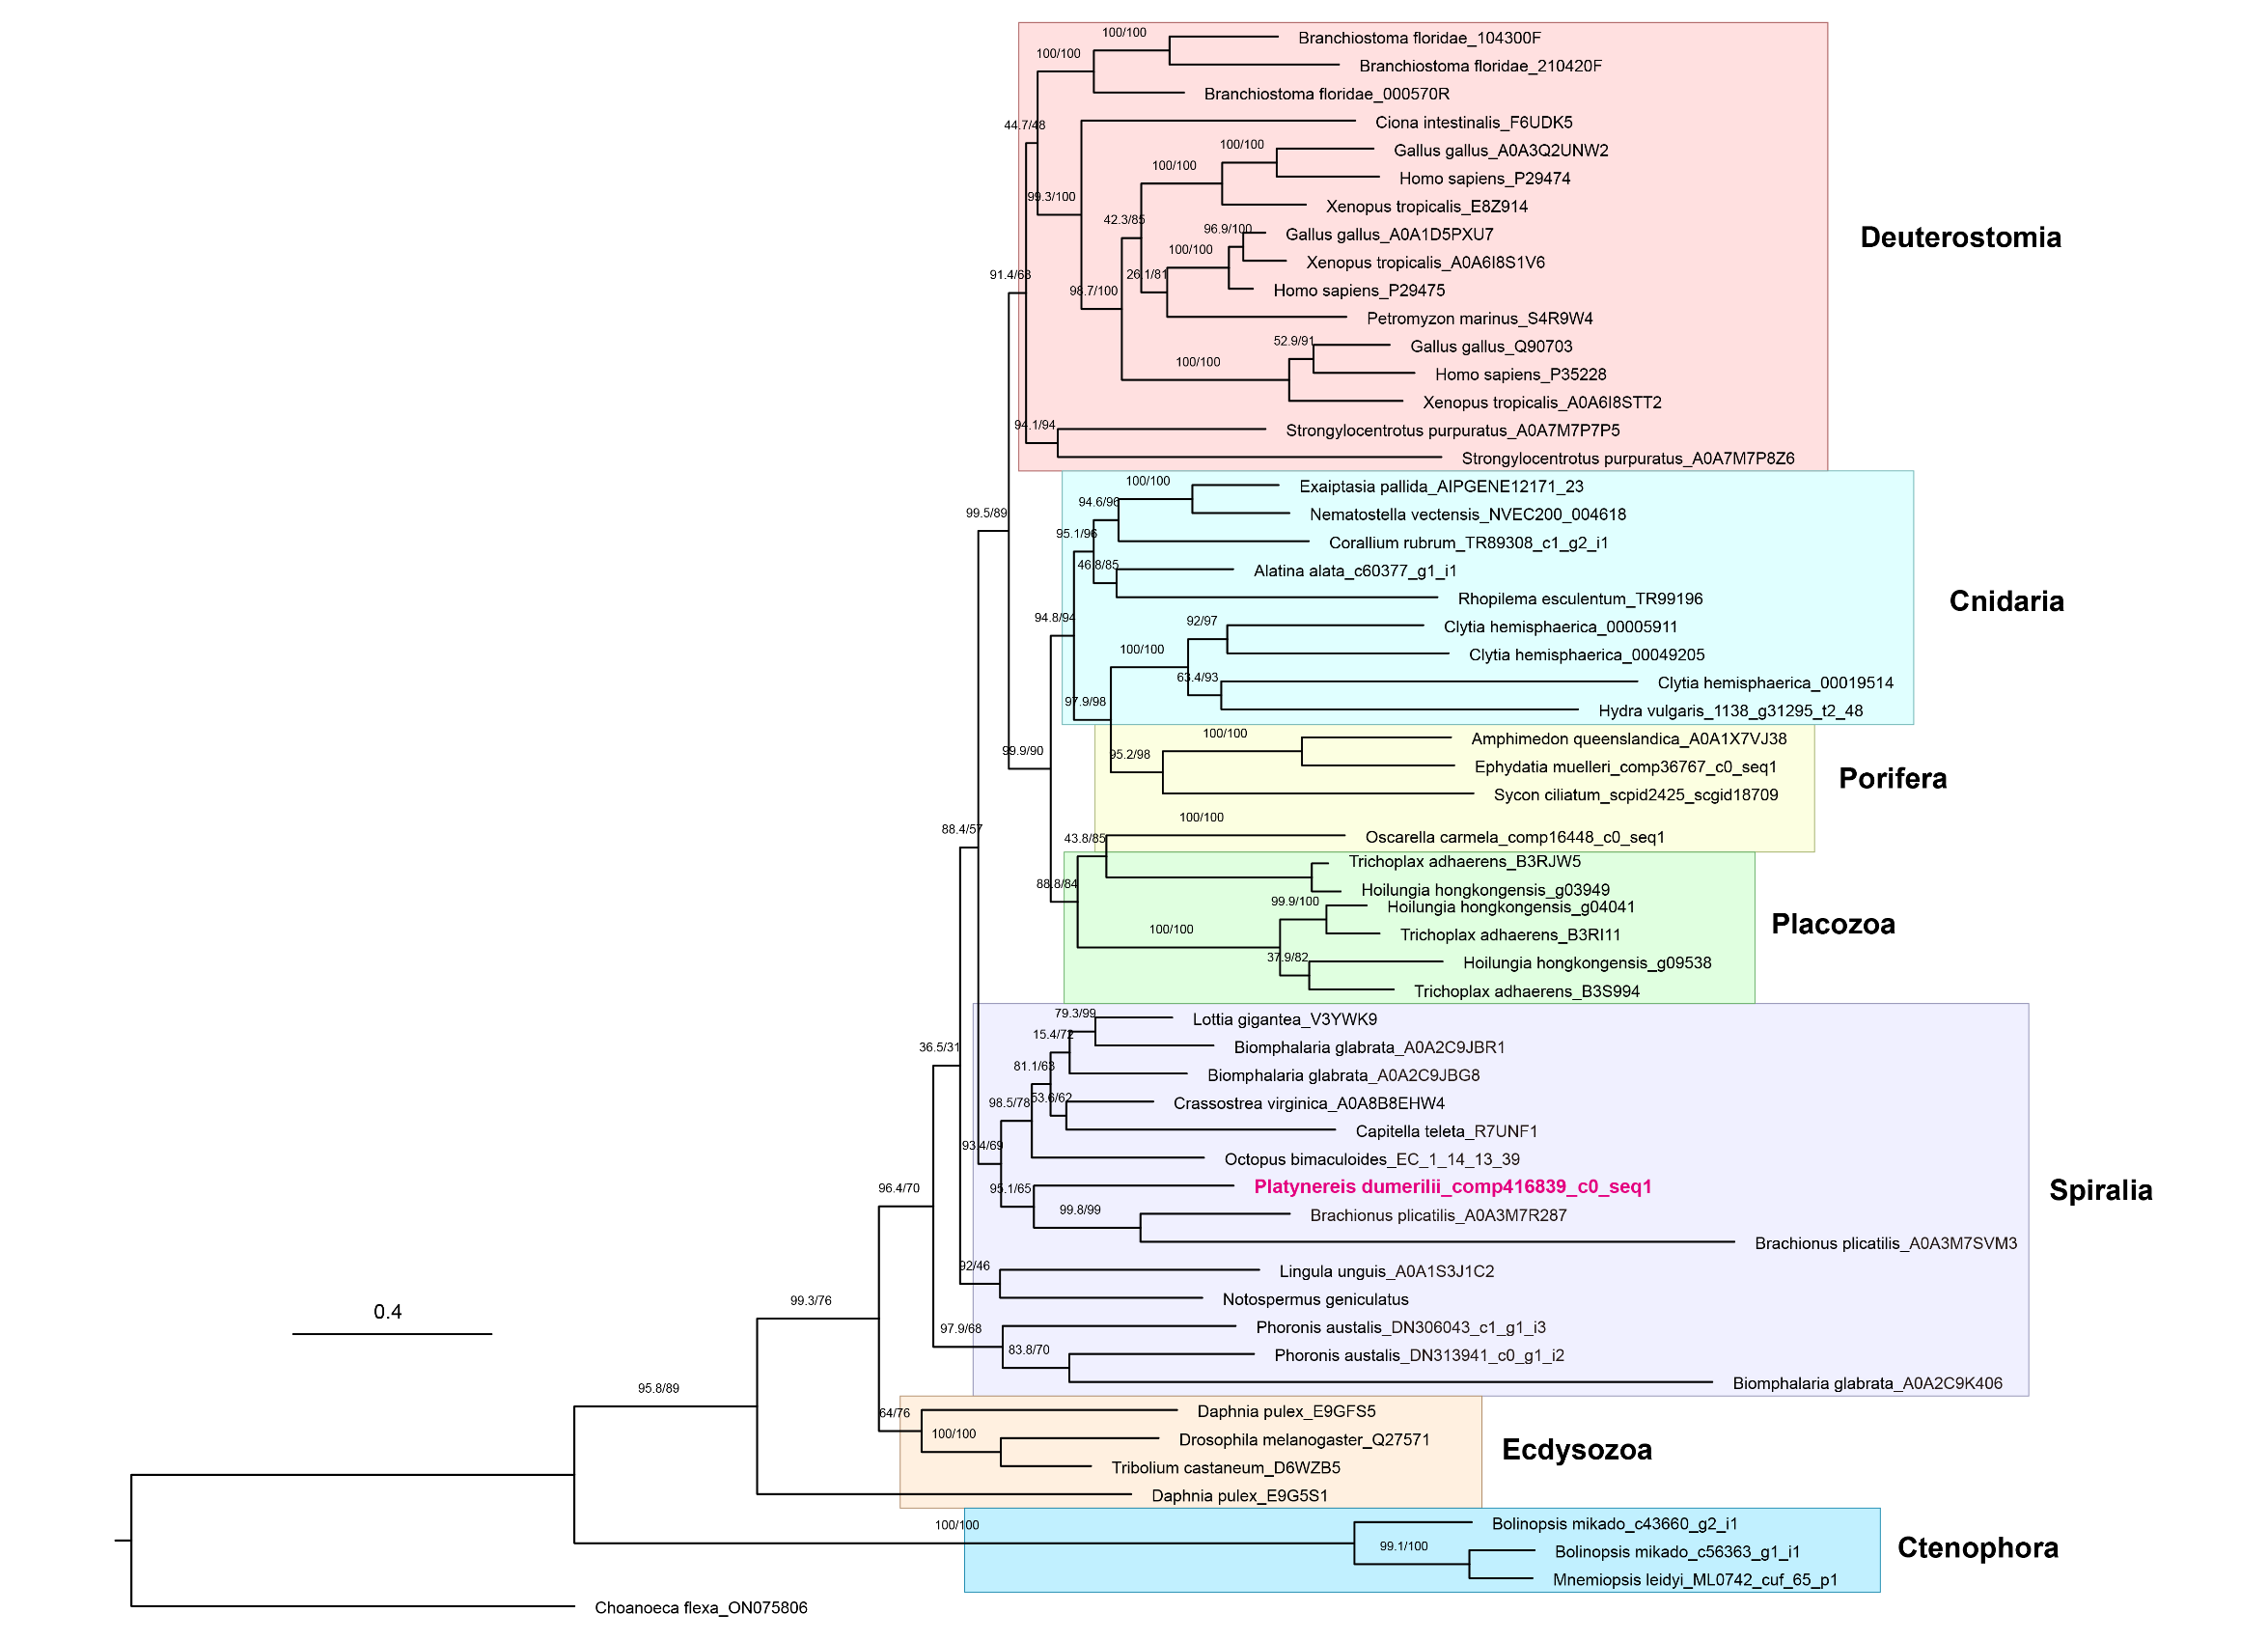
\includegraphics[width=32.64in]{figures/Fig1_sup1} \caption{**Figure 1 -- figure supplement 1**  Phylogenetic tree of NOS by maximum likelihood. Tree robustness was tested with 1000 replicates of ultrafast bootstrap with the aLRT-SH-like and aBayes methods.}\label{fig:unnamed-chunk-8}
\end{figure}

\begin{figure}
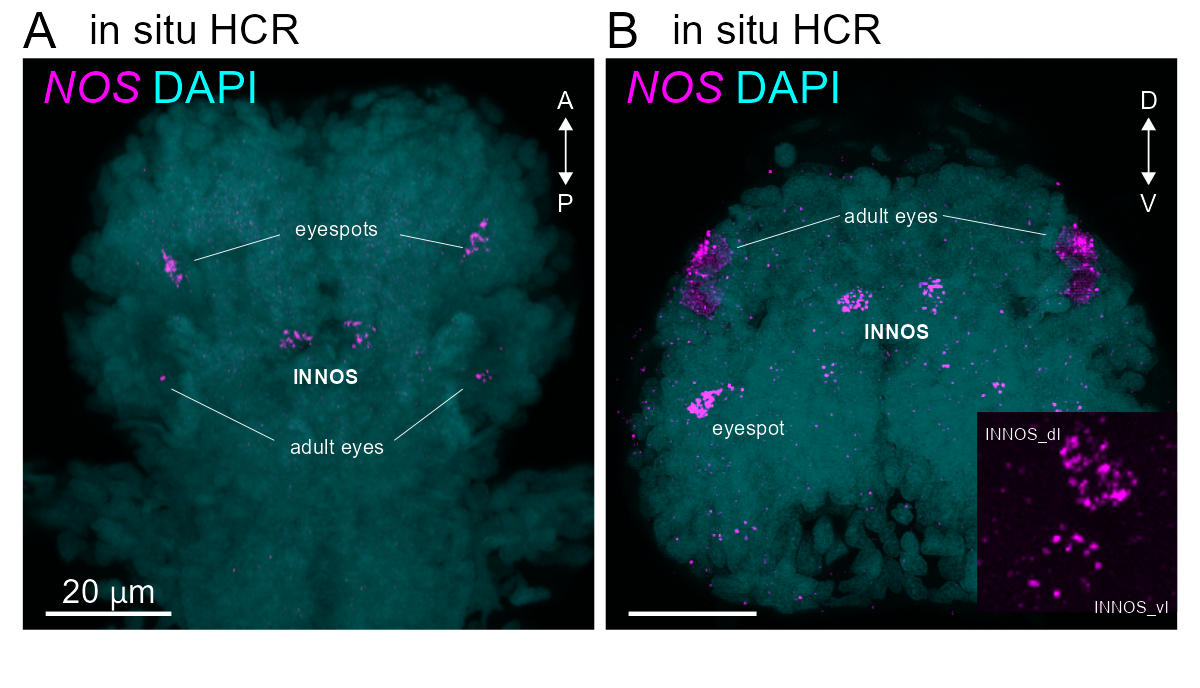
\includegraphics[width=16.67in]{figures/Fig1_sup2} \caption{**Figure 1 -- figure supplement 2** Expression analysis of the *NOS* gene (magenta) using in situ HCR using the larva at three-day-old in dorsal **(A)** and anterior view (B). (B) Insert: showing two NOS cells (INNOS_dl and INNOS_vl) on left side.}\label{fig:unnamed-chunk-9}
\end{figure}

\begin{figure}
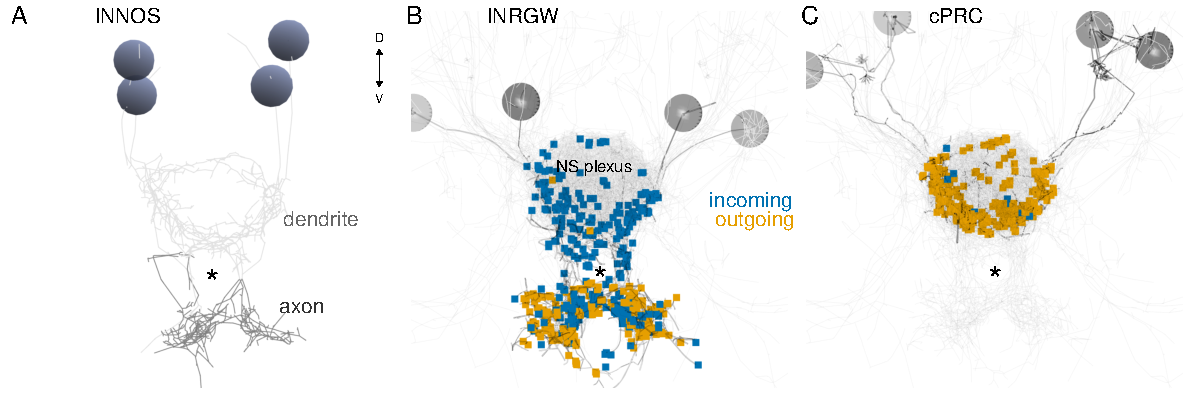
\includegraphics[width=34.72in]{figures/Fig1_sup3} \caption{**Figure 1 -- figure supplement 3** }\label{fig:unnamed-chunk-10}
\end{figure}

\begin{figure}
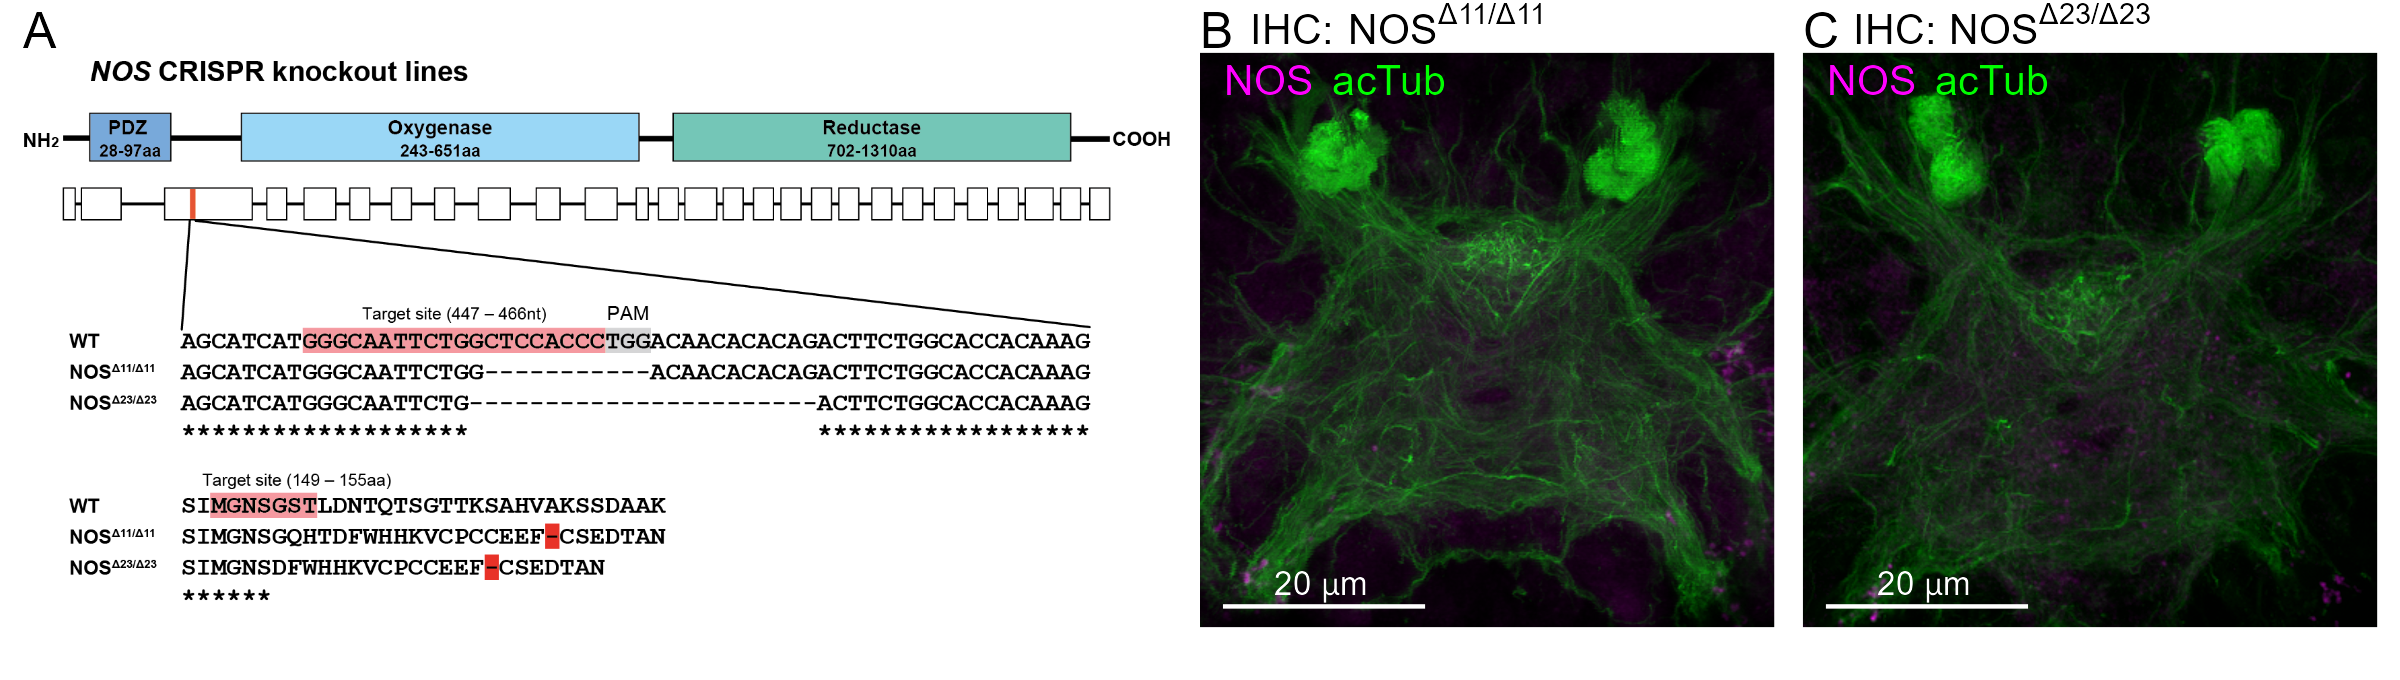
\includegraphics[width=44.44in]{figures/Fig3_sup1} \caption{**Figure 3 -- figure supplement 1** **(A)** Overlaid trajectories for WT (n=37) and NOS mutant (NOSΔ11/Δ11, n=18 and NOSΔ23/Δ23, n=8) at two-day-old larvae. 0 sec as the starting point. After 10 sec, UV (395 nm) stimulation from the side. **(B)** The temporal changes in the vertical position of the WT and mutant 2-days-old larvae before and after UV stimulation are shown. The starting points of each larval trajectory are set to 0. After UV stimulation is indicated by purple squares. **(C)** Vertical swimming in wild-type (WT) and mutant (NOSΔ11 and NOSΔ23) larvae at 2-day-old stimulated with UV (395 nm) light from side, blue (488 nm) light from top and UV (395 nm) light from top. The data are shown in 30 s bins. **(D, E)** The temporal changes in the distance traveled of the WT and mutant in 2-day (D) and 3-day-old (E) larvae before and after UV stimulation are shown.}\label{fig:unnamed-chunk-11}
\end{figure}

\begin{figure}
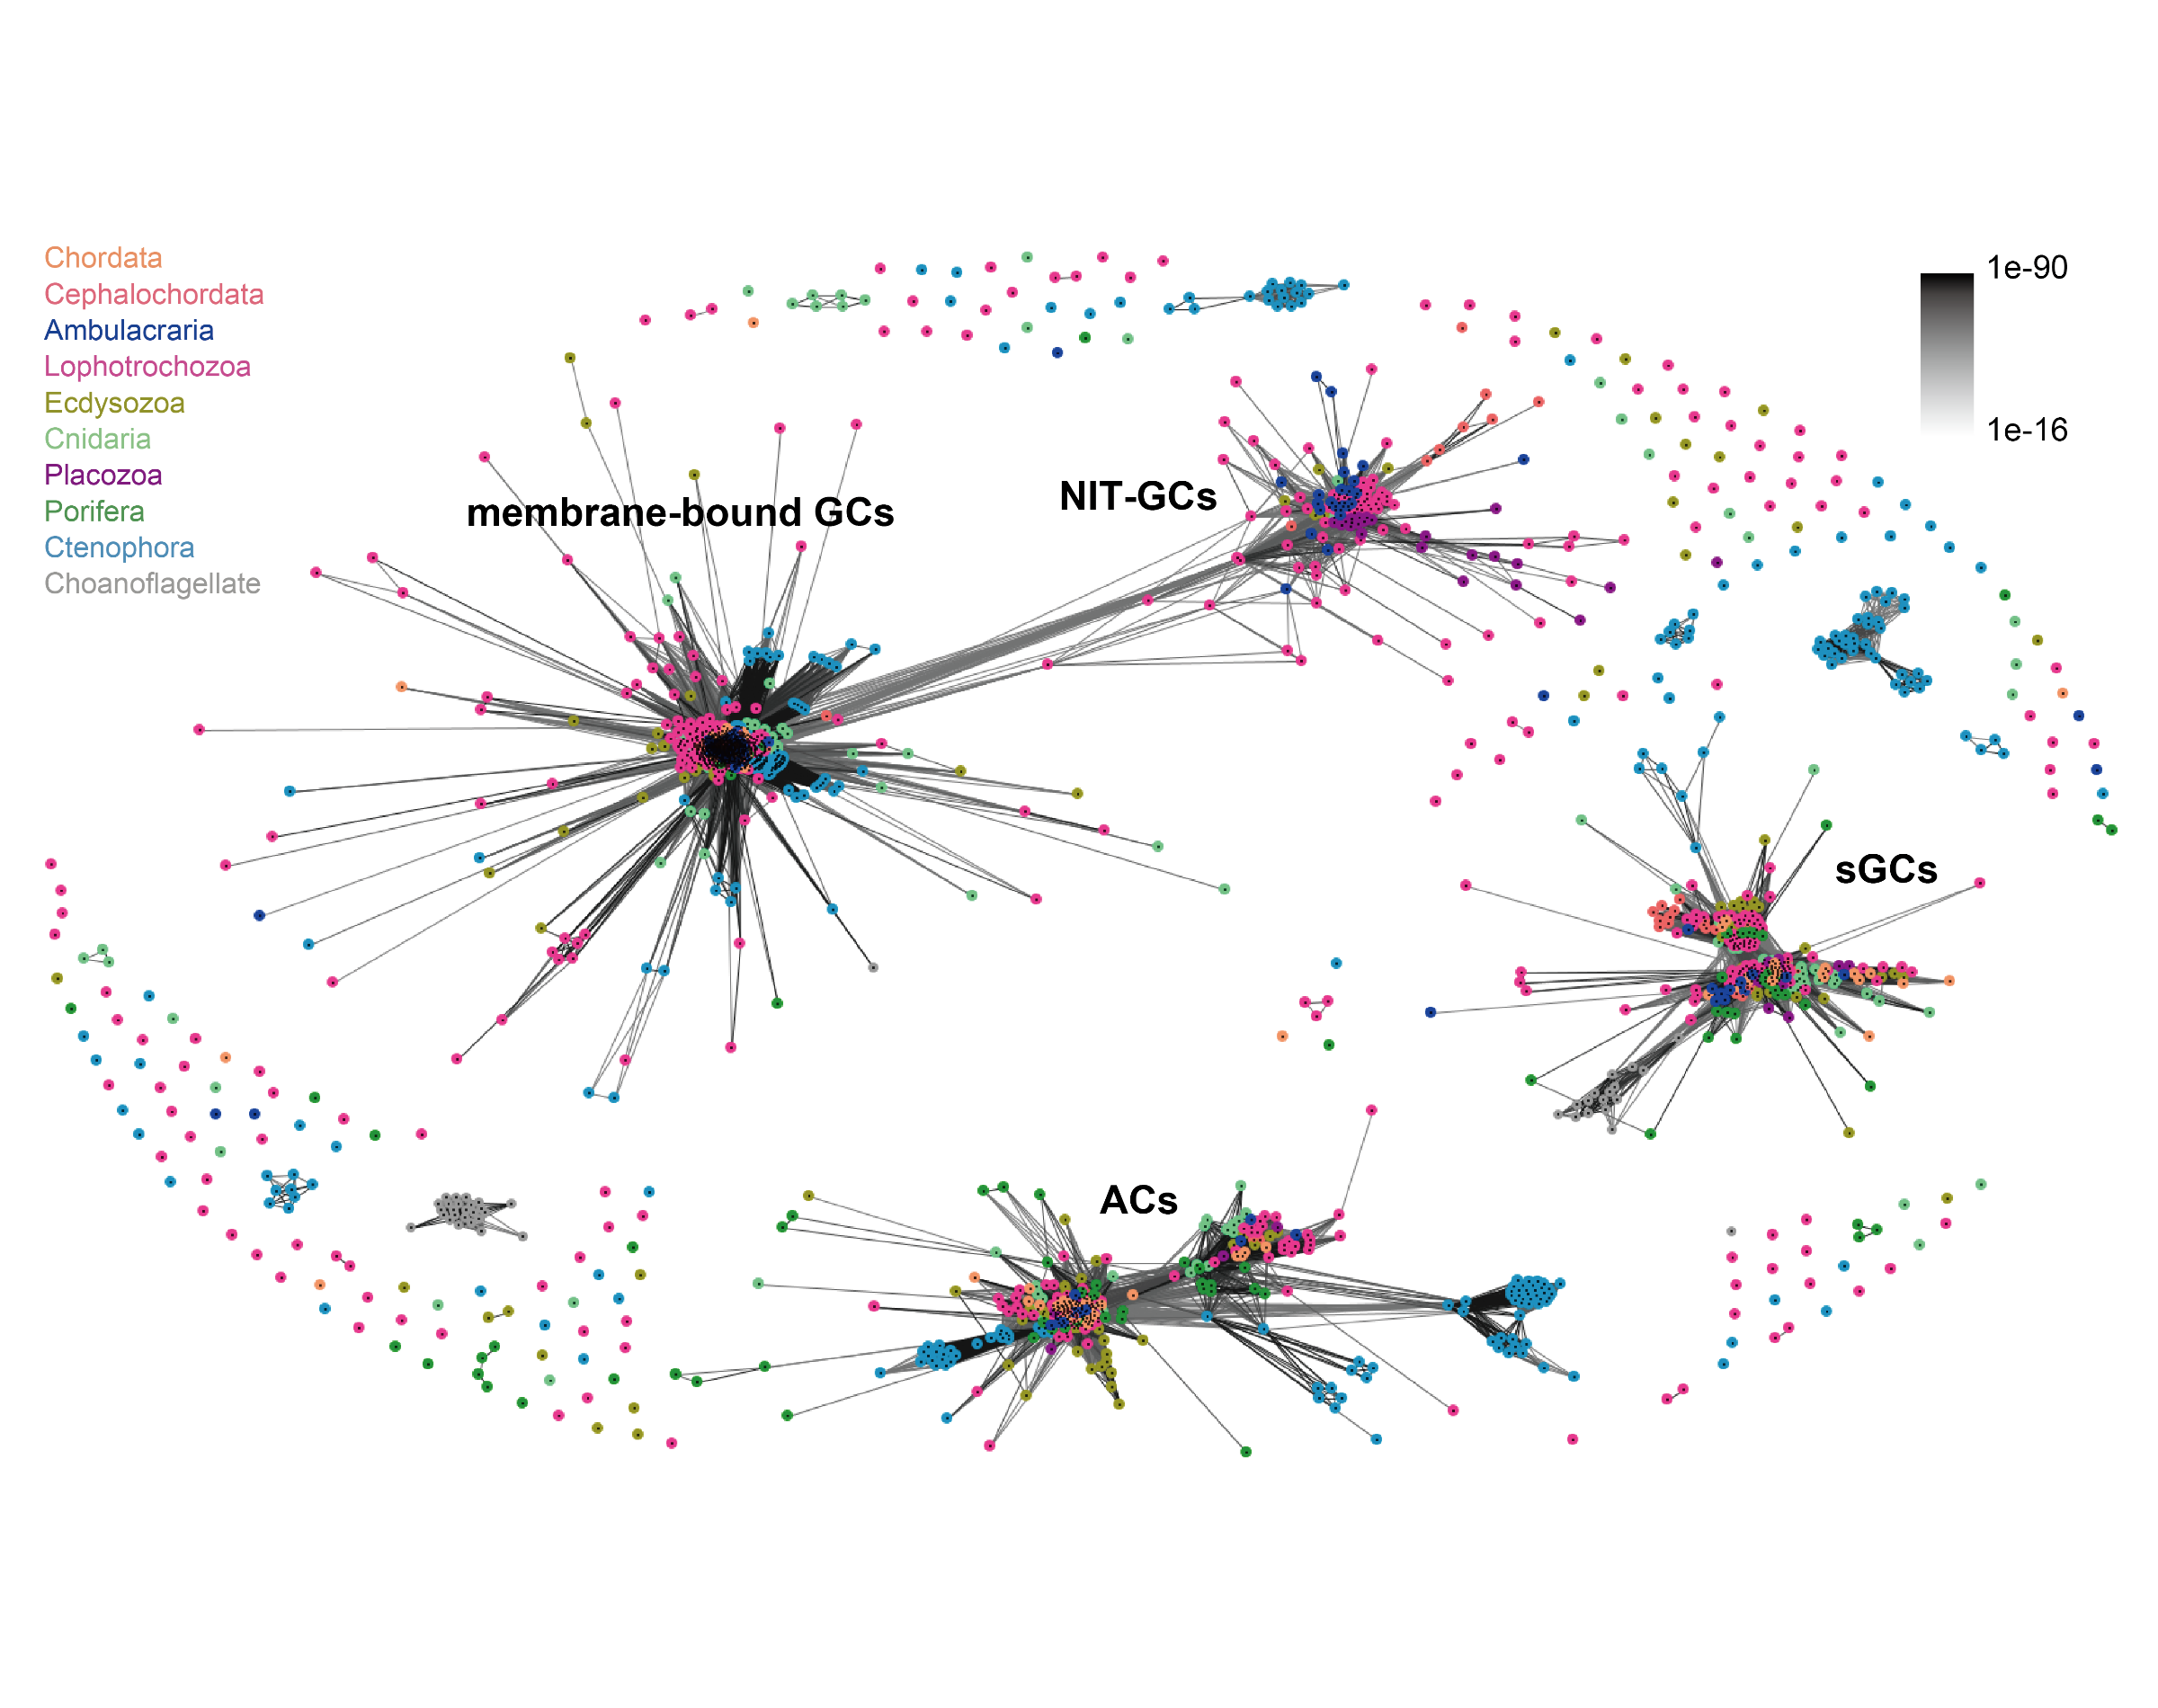
\includegraphics[width=33.33in]{figures/Fig4_sup1} \caption{**Figure 4 -- figure supplement 1** }\label{fig:unnamed-chunk-12}
\end{figure}

\begin{figure}
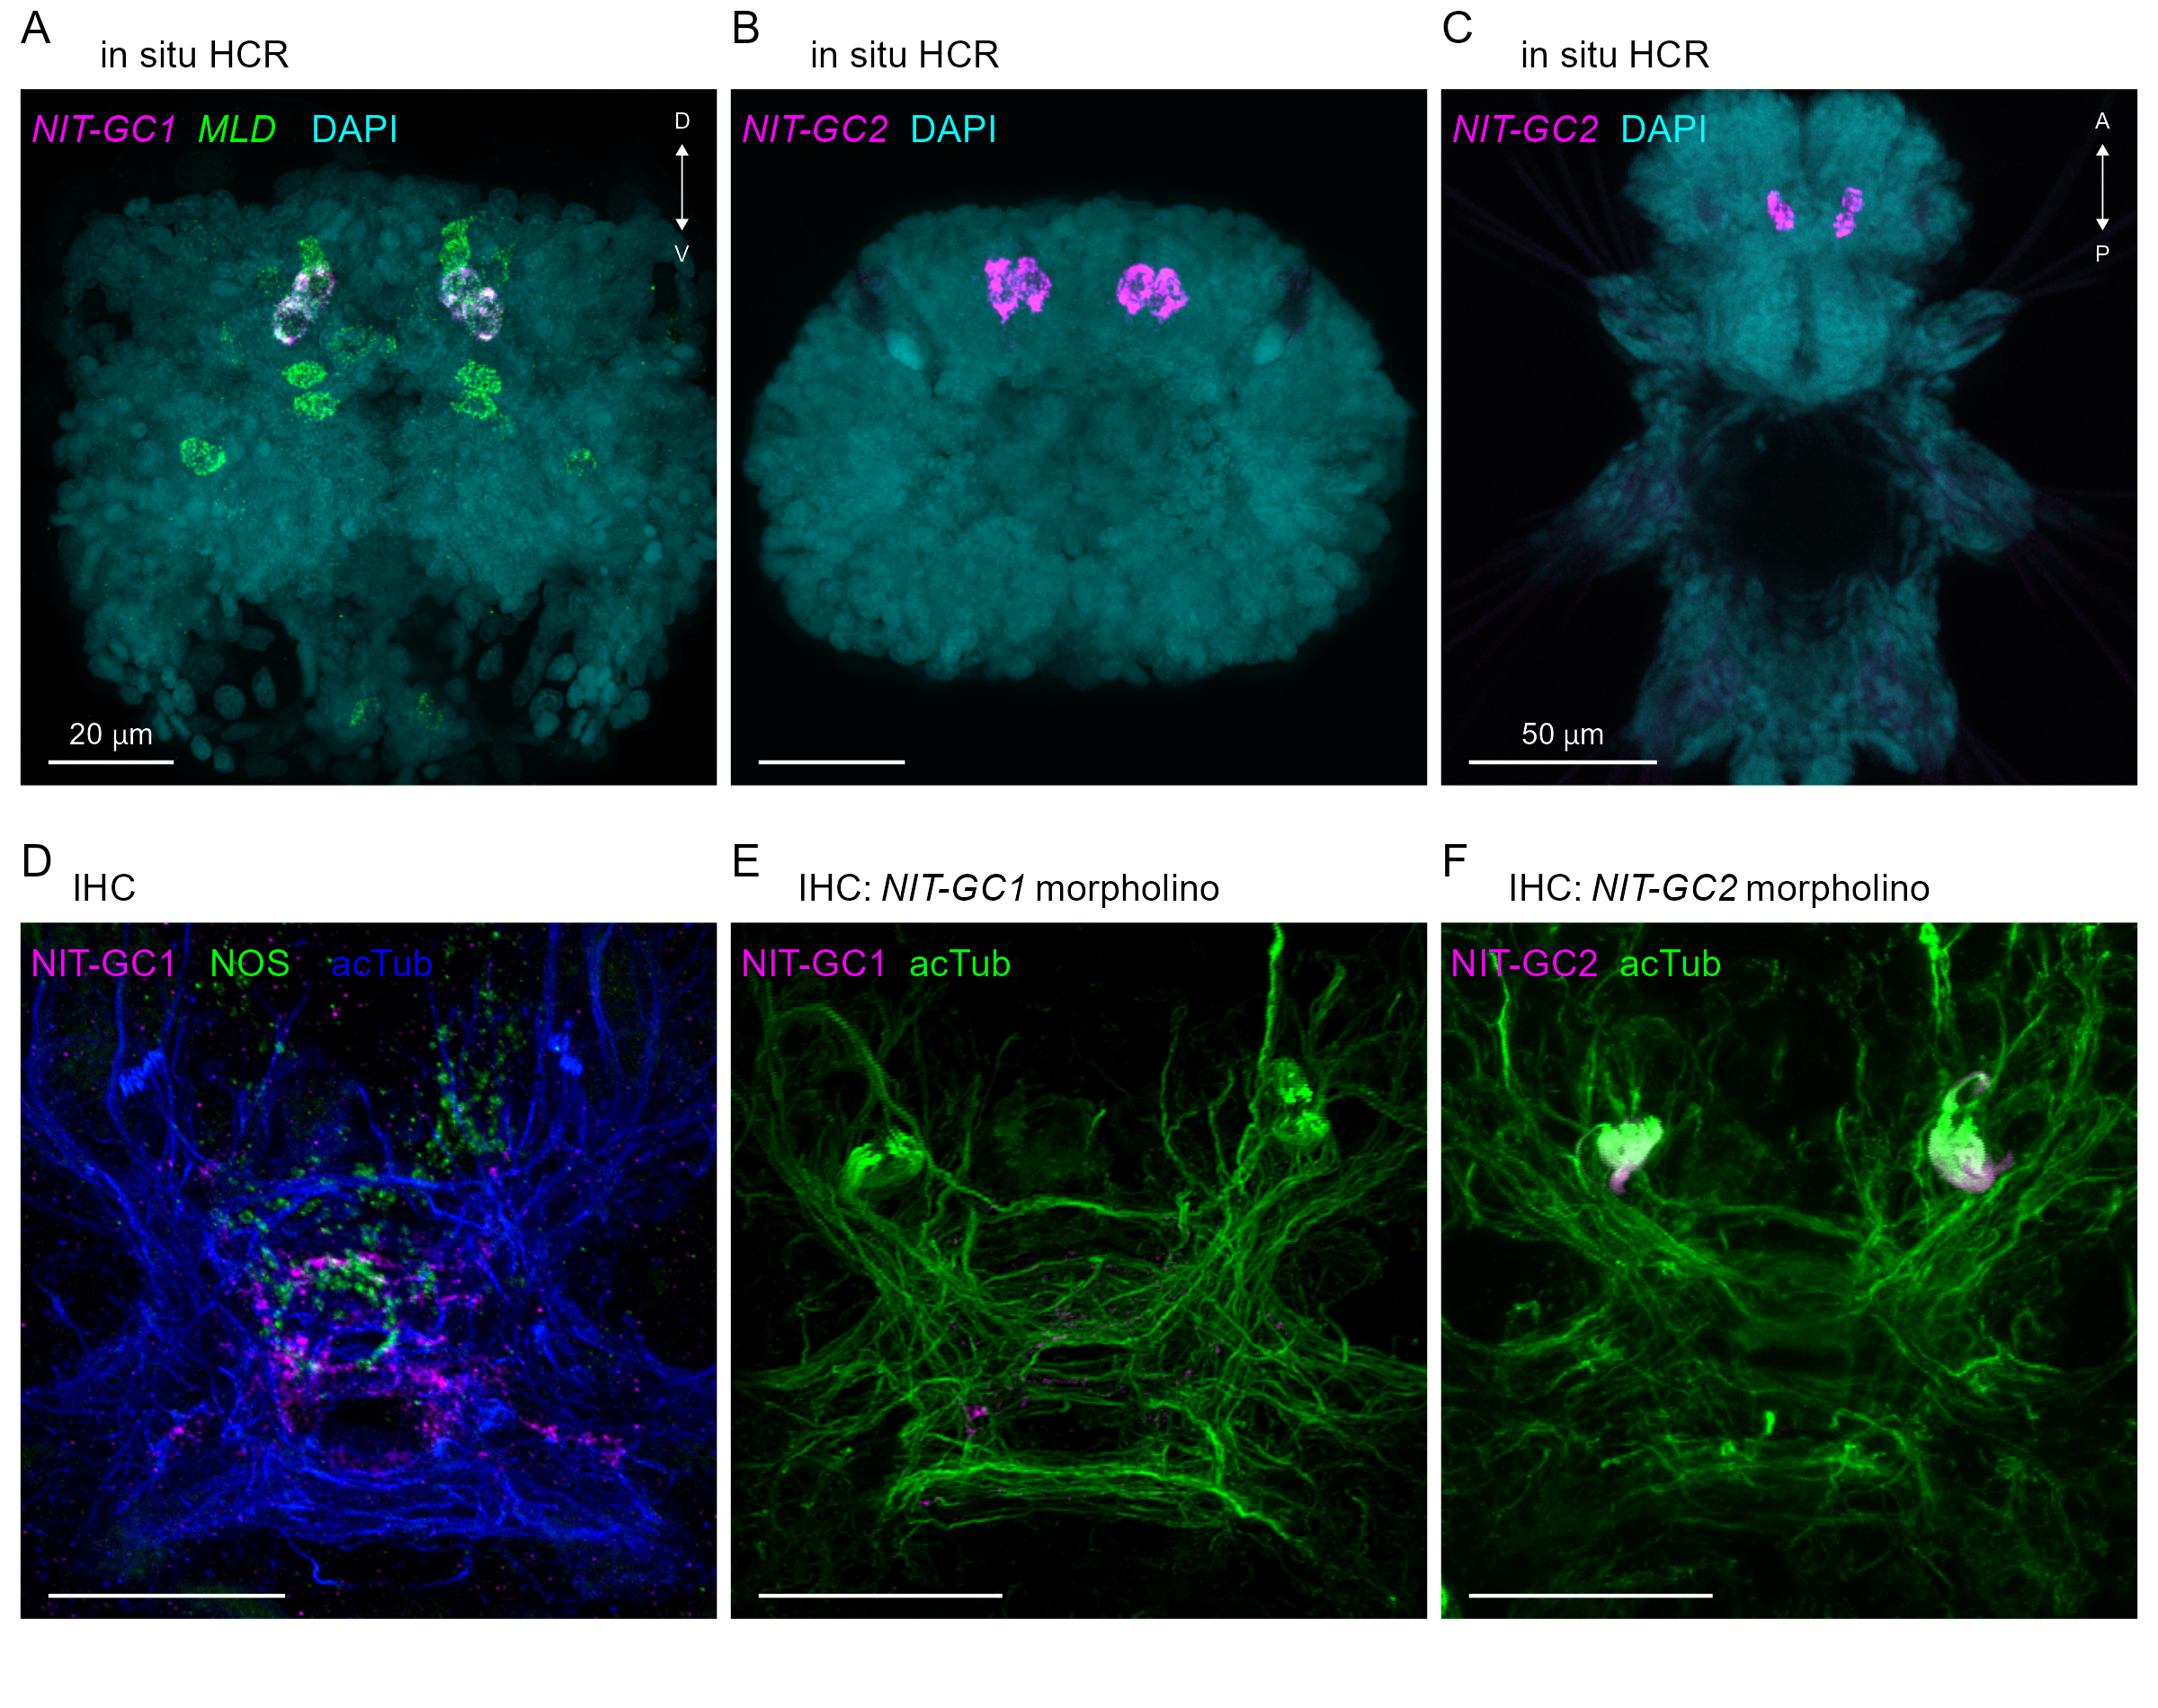
\includegraphics[width=20.83in]{figures/Fig4_sup2} \caption{**Figure 4 -- figure supplement 2** Phylogenetic tree of guanylate cyclase by maximum likelihood (ML). Guanylate cyclase-coupled receptor and soluble guanylate cyclases (sGC) as outgroups. Guanylate cyclases with NIT domains are found in most animal phyla except Porifera, Ctenophora, Urochordata and Chordata. Dot plot of Platynereis NIT-GC genes (columns) expressed in cPRC, INNOS and INRGWa (rows) using single cell RNA-Seq. The size of the dots is expressed in proportion to the percentage of cells expressing that gene relative to all cells. The colours represent the normal logarithm of the number of transcripts in the cells expressing the gene.}\label{fig:unnamed-chunk-13}
\end{figure}

\begin{figure}
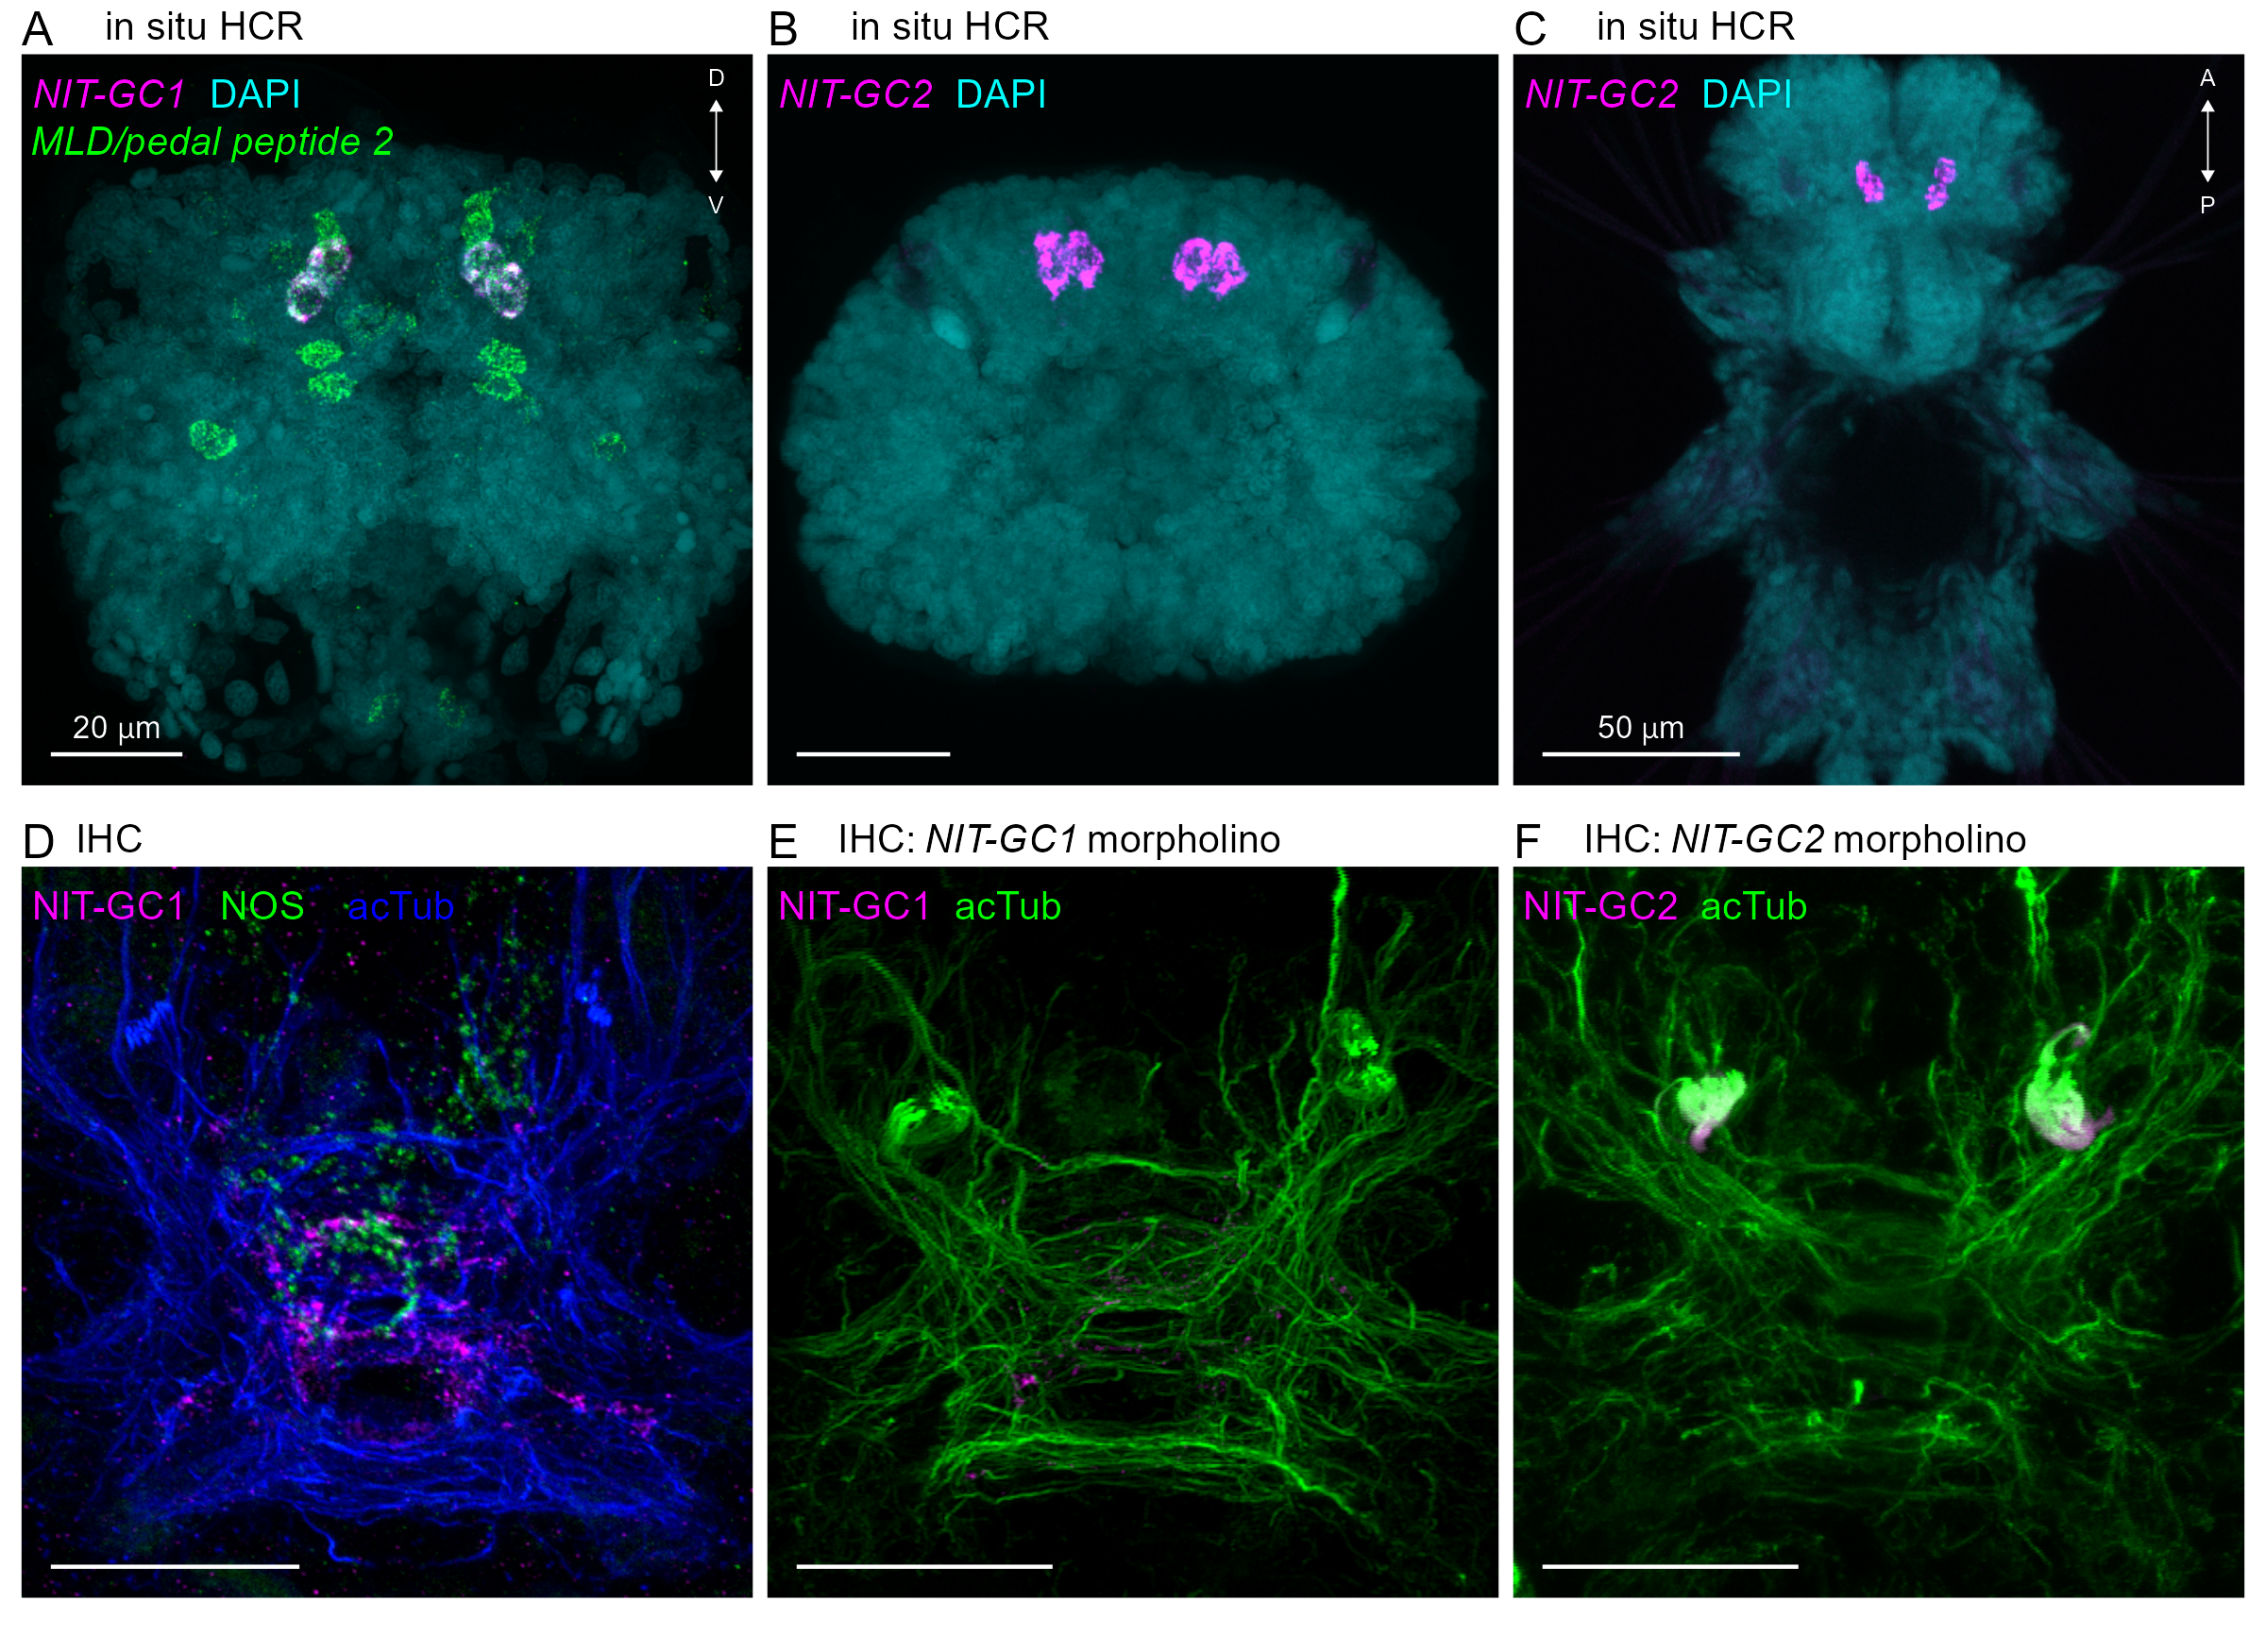
\includegraphics[width=33.33in]{figures/Fig4_sup3} \caption{**Figure 4 -- figure supplement 3** Co-expression analysis image of the NIT-GC1 (magenta) and MLD-pedal2 amide proneuropeptide gene (MLD: green). Anterior view of the larva at two-day-old. **(B, C)** Expression analysis of the NIT-GC2 gene (magenta) using in situ HCR. Anterior (B) and posterior (C) views of the larva at three-day-old. **(D)** Co-localisation analysis using NIT-GC1 (magenta) and NOS (green) antibodies. Anterior view of the larva at two-day-old. **(E, F)** Localisation analysis using NIT-GC1 and NIT-GC2 antibodies for NIT-GC1 (E) and NIT-GC2 (F) morphant. Green shows co-staining with acetylated α-tubulin antibody (acTub). Anterior view of the larva at two-day-old.}\label{fig:unnamed-chunk-14}
\end{figure}

\begin{figure}
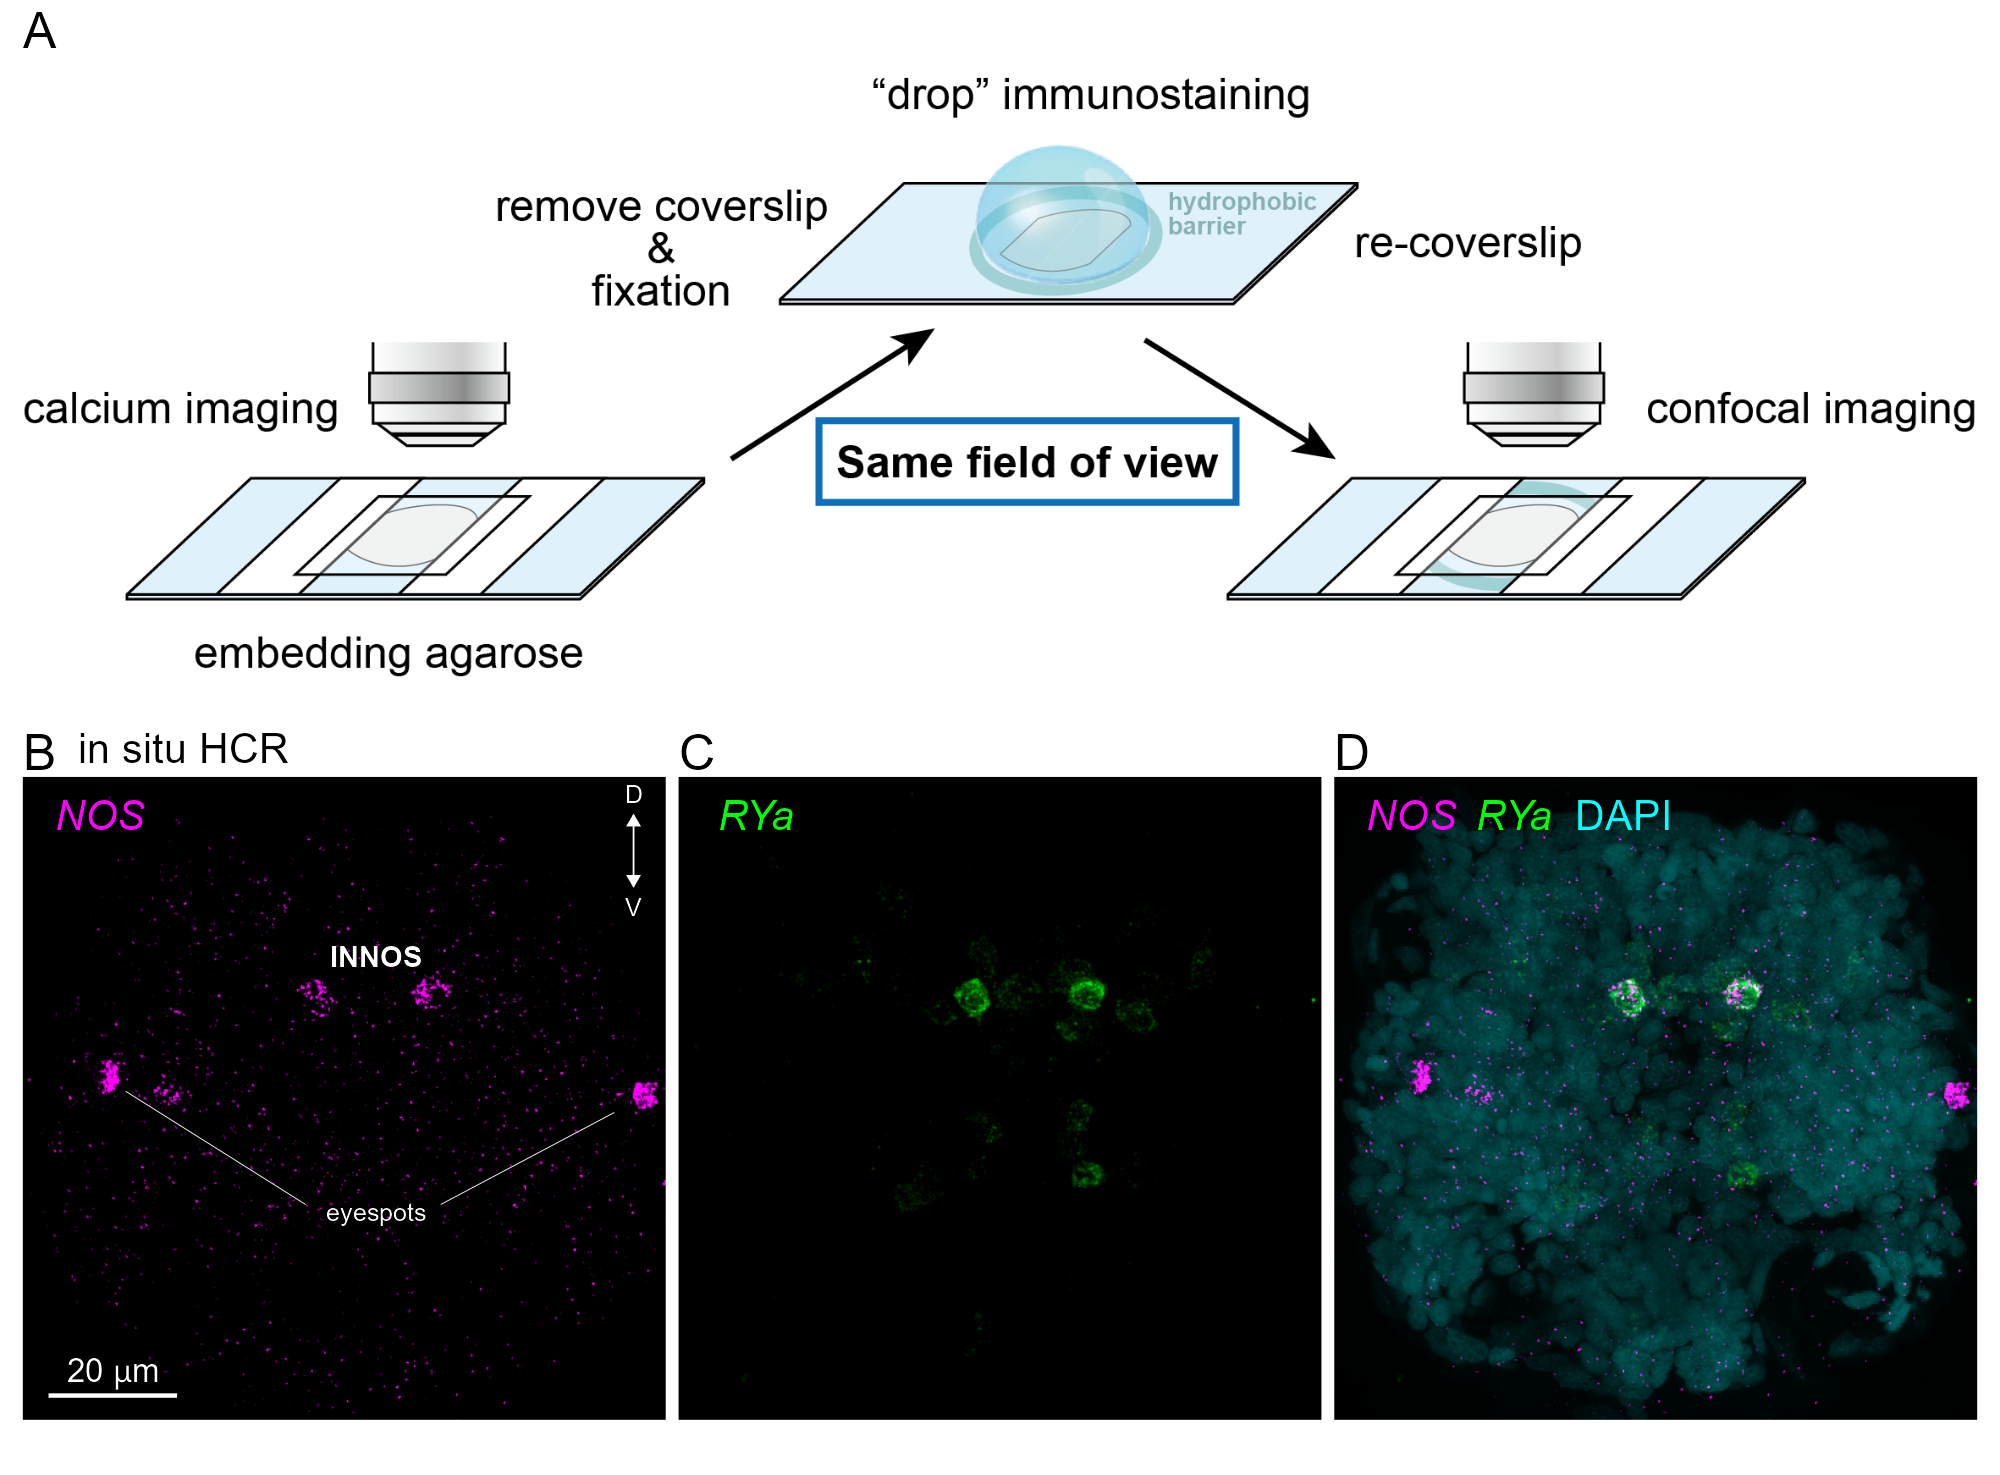
\includegraphics[width=27.78in]{figures/Fig5_sup1} \caption{**Figure 5 -- figure supplement 1** Schematic diagram of the immunostaining procedure after calcium imaging.}\label{fig:unnamed-chunk-15}
\end{figure}

\end{document}
